%File: formatting-instructions-latex-2024.tex
%release 2024.0
\documentclass[letterpaper]{article} % DO NOT CHANGE THIS
\usepackage{aaai24}  % DO NOT CHANGE THIS
\usepackage{times}  % DO NOT CHANGE THIS
\usepackage{helvet}  % DO NOT CHANGE THIS
\usepackage{courier}  % DO NOT CHANGE THIS
\usepackage[hyphens]{url}  % DO NOT CHANGE THIS
\usepackage{graphicx} % DO NOT CHANGE THIS
\urlstyle{rm} % DO NOT CHANGE THIS
\def\UrlFont{\rm}  % DO NOT CHANGE THIS
\usepackage{natbib}  % DO NOT CHANGE THIS AND DO NOT ADD ANY OPTIONS TO IT
\usepackage{caption} % DO NOT CHANGE THIS AND DO NOT ADD ANY OPTIONS TO IT
\frenchspacing  % DO NOT CHANGE THIS
\setlength{\pdfpagewidth}{8.5in}  % DO NOT CHANGE THIS
\setlength{\pdfpageheight}{11in}  % DO NOT CHANGE THIS
%
% These are recommended to typeset algorithms but not required. See the subsubsection on algorithms. Remove them if you don't have algorithms in your paper.
\usepackage{algorithm}
\usepackage{algorithmic}

%
% These are are recommended to typeset listings but not required. See the subsubsection on listing. Remove this block if you don't have listings in your paper.
\usepackage{newfloat}
\usepackage{listings}
\DeclareCaptionStyle{ruled}{labelfont=normalfont,labelsep=colon,strut=off} % DO NOT CHANGE THIS
\lstset{%
	basicstyle={\footnotesize\ttfamily},% footnotesize acceptable for monospace
	numbers=left,numberstyle=\footnotesize,xleftmargin=2em,% show line numbers, remove this entire line if you don't want the numbers.
	aboveskip=0pt,belowskip=0pt,%
	showstringspaces=false,tabsize=2,breaklines=true}
\floatstyle{ruled}
\newfloat{listing}{tb}{lst}{}
\floatname{listing}{Listing}
%
% Keep the \pdfinfo as shown here. There's no need
% for you to add the /Title and /Author tags.

% DISALLOWED PACKAGES
% \usepackage{authblk} -- This package is specifically forbidden
% \usepackage{balance} -- This package is specifically forbidden
% \usepackage{color (if used in text)
% \usepackage{CJK} -- This package is specifically forbidden
% \usepackage{float} -- This package is specifically forbidden
% \usepackage{flushend} -- This package is specifically forbidden
% \usepackage{fontenc} -- This package is specifically forbidden
% \usepackage{fullpage} -- This package is specifically forbidden
% \usepackage{geometry} -- This package is specifically forbidden
% \usepackage{grffile} -- This package is specifically forbidden
% \usepackage{hyperref} -- This package is specifically forbidden
% \usepackage{navigator} -- This package is specifically forbidden
% (or any other package that embeds links such as navigator or hyperref)
% \indentfirst} -- This package is specifically forbidden
% \layout} -- This package is specifically forbidden
% \multicol} -- This package is specifically forbidden
% \nameref} -- This package is specifically forbidden
% \usepackage{savetrees} -- This package is specifically forbidden
% \usepackage{setspace} -- This package is specifically forbidden
% \usepackage{stfloats} -- This package is specifically forbidden
% \usepackage{tabu} -- This package is specifically forbidden
% \usepackage{titlesec} -- This package is specifically forbidden
% \usepackage{tocbibind} -- This package is specifically forbidden
% \usepackage{ulem} -- This package is specifically forbidden
% \usepackage{wrapfig} -- This package is specifically forbidden
% DISALLOWED COMMANDS
% \nocopyright -- Your paper will not be published if you use this command
% \addtolength -- This command may not be used
% \balance -- This command may not be used
% \baselinestretch -- Your paper will not be published if you use this command
% \clearpage -- No page breaks of any kind may be used for the final version of your paper
% \columnsep -- This command may not be used
% % \newpage -- No page breaks of any kind may be used for the final version of your paper
% \pagebreak -- No page breaks of any kind may be used for the final version of your paperr
% \pagestyle -- This command may not be used
% \tiny -- This is not an acceptable font size.
% \vspace{- -- No negative value may be used in proximity of a caption, figure, table, section, subsection, subsubsection, or reference
% \vskip{- -- No negative value may be used to alter spacing above or below a caption, figure, table, section, subsection, subsubsection, or reference

% Extra usepakage
\usepackage{amsmath}
\usepackage{mathtools}
\usepackage{mathrsfs}
\usepackage{amssymb}
\usepackage{booktabs}
%\usepackage{proof-at-the-end}
%\usepackage{xparse}
\usepackage{tablefootnote}
\usepackage{pifont}% http://ctan.org/pkg/pifont
%\usepackage[ruled,vlined,linesnumbered]{algorithm2e}
%\usepackage{comment}
\usepackage[shortlabels]{enumitem}
\setlist[enumerate]{noitemsep, topsep=0pt}
\usepackage{adjustbox}
\usepackage{xspace}
\usepackage{multirow}
\usepackage{amsthm}

\newtheorem{theorem}{Theorem}
\newtheorem{lemma}{Lemma}
\newtheorem{proposition}{Proposition}
\newtheorem{definition}{Definition}
\newtheorem{assumption}{Assumption}
\newtheorem{remark}{Remark}
\newtheorem{corollary}{Corollary}
\usepackage{color}
\newcommand{\red}[1]{\begin{color}{red}#1\end{color}}

\setcounter{secnumdepth}{0} %May be changed to 1 or 2 if section numbers are desired.

% The file aaai24.sty is the style file for AAAI Press
% proceedings, working notes, and technical reports.
%

% Title

% Your title must be in mixed case, not sentence case.
% That means all verbs (including short verbs like be, is, using,and go),
% nouns, adverbs, adjectives should be capitalized, including both words in hyphenated terms, while
% articles, conjunctions, and prepositions are lower case unless they
% directly follow a colon or long dash
\title{A Bregman Proximal Stochastic Gradient Method with Extrapolation for Nonconvex Nonsmooth Problems}
\author{
	%Authors
	% All authors must be in the same font size and format.
	%Written by AAAI Press Staff\textsuperscript{\rm 1}\thanks{With help from the AAAI Publications Committee.}\\
	%AAAI Style Contributions by Pater Patel Schneider,
	%Sunil Issar,\\
	%J. Scott Penberthy,
	%George Ferguson,
	%Hans Guesgen,
	%Francisco Cruz\equalcontrib,
	%Marc Pujol-Gonzalez\equalcontrib
	Qingsong Wang\textsuperscript{\rm 1},
	Zehui Liu\textsuperscript{\rm 2},
	Chunfeng Cui\textsuperscript{\rm 2}\thanks{Corresponding author.},
	Deren Han\textsuperscript{\rm 2}
}
\affiliations{
	%Afiliations
	\textsuperscript{\rm 1}School of Mathematics and Computational Science, Xiangtan University, China\\
	\textsuperscript{\rm 2}LMIB, School of Mathematical Sciences, Beihang University, China\\
	nothing2wang@hotmail.com, \{liuzehui, chunfengcui, handr\}@buaa.edu.cn
	% If you have multiple authors and multiple affiliations
	% use superscripts in text and roman font to identify them.
	% For example,

	% Sunil Issar\textsuperscript{\rm 2},
	% J. Scott Penberthy\textsuperscript{\rm 3},
	% George Ferguson\textsuperscript{\rm 4},
	% Hans Guesgen\textsuperscript{\rm 5}
	% Note that the comma should be placed after the superscript

	%1900 Embarcadero Road, Suite 101\\
	%Palo Alto, California 94303-3310 USA\\
	% email address must be in roman text type, not monospace or sans serif
	%proceedings-questions@aaai.org
	%
	% See more examples next
}

%Example, Single Author, ->> remove \iffalse,\fi and place them surrounding AAAI title to use it
\iffalse
\title{My Publication Title --- Single Author}
\author {
	Author Name
}
\affiliations{
	Affiliation\\
	Affiliation Line 2\\
	name@example.com
}
\fi

\iffalse
%Example, Multiple Authors, ->> remove \iffalse,\fi and place them surrounding AAAI title to use it
\title{My Publication Title --- Multiple Authors}
\author {
	% Authors
	First Author Name\textsuperscript{\rm 1,\rm 2},
	Second Author Name\textsuperscript{\rm 2},
	Third Author Name\textsuperscript{\rm 1}
}
\affiliations {
	% Affiliations
	\textsuperscript{\rm 1}Affiliation 1\\
	\textsuperscript{\rm 2}Affiliation 2\\
	firstAuthor@affiliation1.com, secondAuthor@affilation2.com, thirdAuthor@affiliation1.com
}
\fi


% REMOVE THIS: bibentry
% This is only needed to show inline citations in the guidelines document. You should not need it and can safely delete it.
%\usepackage{bibentry}
% END REMOVE bibentry

\begin{document}

	\maketitle

	\begin{abstract}
		In this paper, we explore a specific optimization problem that involves the combination of a differentiable nonconvex function and a nondifferentiable function. The differentiable component lacks a global Lipschitz continuous gradient, posing challenges for optimization.  To address this issue and accelerate the convergence, we propose a Bregman proximal stochastic gradient method with extrapolation (BPSGE), which only requires smooth adaptivity of the differentiable part.  Under the variance reduction framework, we not only analyze the subsequential and global convergence of the proposed algorithm under certain conditions,  but also analyze the sublinear convergence rate of the subsequence, and the complexity of the algorithm, revealing that the BPSGE algorithm requires at most  $\mathcal{O}(\varepsilon^{-2})$ iterations in expectation to attain an $\varepsilon$-stationary point.  To validate the effectiveness of our proposed algorithm, we conduct numerical experiments on three real-world applications: graph regularized nonnegative matrix factorization (NMF), matrix factorization with weakly-convex regularization, and NMF with nonconvex sparsity constraints. These experiments demonstrate that BPSGE is faster than the baselines without extrapolation.
	\end{abstract}

	\section{Introduction}
	In this paper, we  consider the following nonsmooth nonconvex optimization problem
	\begin{eqnarray}
		\min_{x\in \overline{C}}\quad \Phi(x):=f(x)+h(x), \label{target_function}
	\end{eqnarray}
	where $\overline{C}$ denotes the closure of $C$, which is a nonempty, convex, and open set in $\mathbb{R}^{d}$, $f$ is a continuously differentiable  (may be nonconvex) function which can be written as $f(x)=\frac{1}{n}\sum_{i=1}^{n}f_{i}(x)$, and $h$ is an extended valued function (maybe nonconvex), which is a regularizer promoting low-complexity structures such as sparsity \cite{Donoho95, FanL01, Zhang10} or non-negativity \cite{LeeS99, HeXZZC11} in the solution. Throughout this paper, the usual restrictive requirement of global Lipschitz continuity of the gradient of $f$ is not needed  \cite{Lan2020First, Gillis20}. Many applications can be categorized in the optimization problem \eqref{target_function}, such as matrix and tensor factorization \cite{ComonGLM08, KoldaB09, CheW20}, supervised neural network model \cite{HasannasabHNPSS2020},  and Poisson deconvolution/inverse problems \cite{BolteSTV18First}.

	\textbf{Deterministic Bregman type methods.} The Bregman proximal gradient (BPG) algorithm \cite{BolteSTV18First} is a state-of-the-art method for addressing optimization problems characterized by the absence of global  Lipschitz continuous gradients. It is simple and far-reaching,
	%and based on adapting the geometry to the objective through the Bregman distance paradigm. Specifically, this paradigm involves substituting
	which substitutes the customary upper quadratic approximation of a smooth function with a more comprehensive proximity measure \cite{BauschkeBT17}.  Zhang et al. \cite{ZhangBM0C19} proposed an extrapolation version of the BPG algorithm, denoted by BPGE, under the assumption that  $h(x)$ is convex. Recently, Mukkamala et al. \cite{MukkamalaOPS20} introduced an inertial variant of the BPG method, referred to as the CoCaIn BPG algorithm, which tunes the inertial parameter by convex-concave backtracking.
	%This backtracking strategy capitalizes on the ability to construct both lower and upper approximations for smooth adaptable functions.
	Compared with the original BPG method \cite{BolteSTV18First}, the CoCaIn BPG algorithm exhibits superior numerical performance.
	Moreover, the BPG framework facilitates the discovery of novel techniques tailored to specific problem domains. For instance,  Teboulle and Vaisbourd \cite{TeboulleV20} explored new decomposition settings of the nonnegative matrix factorization (NMF) problem with sparsity constraints. Additionally, an alternative perspective is to consider the BPG-type algorithm by the splitting method. Ahookhos et al. \cite{AhookhoshTP21} proposed a Bregman forward-backward splitting line search method, which demonstrates locally superlinear convergence to nonisolated local minima by leveraging the Bregman forward-backward envelope \cite{BauschkeDL18, LaudeOC20}. Furthermore, Wang et al. \cite{WangTOW22} investigated a Bregman and inertial extension of the forward-reflected-backward algorithm \cite{MalitskyT20} under relative smoothness conditions. %This extension involves incorporating inertial steps in the dual space and allows for the consideration of potentially negative inertial values.
	Numerous other works have explored the Bregman gradient method framework to tackle the absence of global  Lipschitz continuous gradients, including  \cite{ReemRP19, ZhaoDRW22, ZhuDLZ21, DragomirTdB22}.



	\begin{table*}[!ht]
		\centering
		\begin{adjustbox}{max width=\textwidth}
			\begin{tabular}{c|c| c| c |c |c}\hline
				Versions& Algorithm&$h(x)$&Inertial&Sequence convergence &  Complexity\cr\hline
				\multirow{6}{*}{Deterministic} & BPG \cite{BolteSTV18First}& nonconvex & no &subsequential/global &-\\\cline{2-6}
				&BPGE \cite{ZhangBM0C19}& convex &yes & subsequential/global &- \\\cline{2-6}
				& CoCaIn BPG \cite{MukkamalaOPS20}& weakly-convex &yes & subsequential/global &- \\\cline{2-6}
				& BBPG \cite{TeboulleV20} & nonconvex & no &global& -\\\cline{2-6}
				& $i^{*}$FRB \cite{WangTOW22} & nonconvex &no & global&- \\\cline{2-6}
				& BELLA \cite{AhookhoshTP21}& nonconvex &no & subsequential/global&-\\\hline
				\multirow{5}{*}{Stochastic} & SMD \cite{ZhangH18} & convex & no &- & $\mathcal{O}(\varepsilon^{-2})$\\\cline{2-6}
				& SVRAMD \cite{LiWZC22} & convex &no &  - & $\mathcal{O}(n\varepsilon^{-\frac{2}{3}}+\varepsilon^{-\frac{5}{3}})$\\\cline{2-6}
				&BFinito \cite{LatafatTAP22} & nonconvex  & no & subsequential/global &-\\\cline{2-6}
				& BPSG \cite{WangH23} & nonconvex & no &subsequential/global  & - \\\cline{2-6}
				& BPSGE (Algorithm \ref{BPSGE}) & weakly-convex & yes &subsequential/global  & $\mathcal{O}(\varepsilon^{-2})$\\\hline
			\end{tabular}
		\end{adjustbox}
		\caption{Summary of the properties of BPSGE (Algorithm \ref{BPSGE}) and several state-of-the-art methods. ``Complexity'' means the complexity (in expectation) to obtain an $\varepsilon$-stationary point (Definition \ref{stationary-point}) of $\Phi$ and ``-'' means not given.}
		\label{results}
	\end{table*}


	\textbf{Stochastic Bregman type methods.} For large-scale datasets, the cost associated with computing the full gradient can become prohibitively high.  To address this concern, the full gradient can be replaced with a stochastic gradient estimator \cite{RobbinsM1951, Bottou10} which has yielded remarkable achievements in the field of machine learning \cite{LinLF2020book, Lan2020First}. For the optimization problem without the global  Lipschitz continuous gradients, Zhang and He \cite{ZhangH18} conducted a study on the non-asymptotic stationary convergence behaviour of stochastic mirror descent under certain conditions.  In a similar vein, Li et al. \cite{LiWZC22} proposed a simple and generalized algorithmic framework for incorporating variance reduction into adaptive mirror descent algorithms. However, both approaches \cite{ZhangH18, LiWZC22} require $h(\cdot)$ to be a convex function. To address the limitations posed by convexity assumptions, Latafat et al. \cite{LatafatTAP22} introduced a  Bregman incremental aggregated method that extends the Finito/MISO techniques\cite{DefazioDC14, Mairal15} to non-Lipschitz and nonconvex scenarios. However, it is noteworthy that this approach is memory-intensive and demands periodic computation of the full gradient, which is expensive for large-scale problems. Furthermore, the analysis carried out by Latafat et al. \cite{LatafatTAP22} only encompasses two specific variance reduction stochastic estimators, raising doubts about the generalizability of the convergence results to other estimators. To address the aforementioned concerns,  Wang and Han \cite{WangH23} introduced a stochastic version of the BPG algorithm \cite{BolteSTV18First}, known as the Bregman proximal stochastic gradient (BPSG) method which does not assume $h(\cdot)$ is convex. Under a general framework of variance reduction, they also established the convergence properties of the generated sequence in terms of subsequential and global convergence.

	A summary of the aforementioned algorithms is presented in Table \ref{results}.

	Notwithstanding the notable advancements, there remain areas that warrant further improvement.  Firstly,
	%the complexity  analysis for the proposed algorithms \cite{LatafatTAP22, WangH23} has not been addressed when $h(\cdot)$ is nonconvex.
	when $h(\cdot)$ is nonconvex, existing stochastic methods such as BFinito \cite{LatafatTAP22} and BPSG \cite{WangH23}   only analyzed the subsequence and global convergence of the proposed algorithms, yet the sublinear convergence rate of the subsequence and the complexity of the algorithms are unknown.
	Secondly, the accelerated versions of the Bregman stochastic gradient methods  %in \cite{ZhangH18, LiWZC22, LatafatTAP22, WangH23}
	have not been taken into account.
	%From numerical experiments
	Numerically, the incorporation of accelerated techniques, such as the heavy ball \cite{Polyak64} and the Nesterov acceleration \cite{Nesterov1983}, with BPSG can further accelerate the numerical performance \cite{LinLF2020book}.


	In this paper, we introduce the Bregman proximal stochastic gradient method with extrapolation (BPSGE) to solve the nonconvex nonsmooth optimization problem \eqref{target_function}. Our main contributions addressed in this article are as follows:
	\begin{itemize}
		\item With a general variance reduction framework (see Definition \ref{vr_definition}), we establish the sublinear convergence rate for the subsequence %subsequential sequence
		generated by the proposed algorithm.
		\item Under the assumption of $C=\mathbb{R}^{d}$, we show that the BPSGE algorithm  requires at most $\mathcal{O}(\varepsilon^{-2})$ iterations in expectation to attain an $\varepsilon$-stationary point. Additionally, we establish the global convergence of the {sequence} generated by   BPSGE, leveraging the Kurdyka-{\L}ojasiewicz (K{\L}) property.
		\item Numerical experiments are conducted on three distinct problems: graph regularized NMF, matrix factorization (MF) with weakly-convex regularization, and  NMF with nonconvex sparsity constraints. The results of these experiments highlight the favourable performance and enhanced efficiency of the BPSGE algorithm when compared to corresponding algorithms without extrapolation.
	\end{itemize}

	The rest of this paper is organized as follows. Section \ref{preliminary} provides some relevant definitions and results. We present a detailed formulation of the BPSGE algorithm and prove its convergence and convergence rate results in Section \ref{algorithm} and Section \ref{convergence_analysis}, respectively. In Section \ref{numercial_experiments} we use three applications to compare BPSGE with several other algorithms. Finally, we draw conclusions in Section \ref{conclusion}.


	\section{Preliminary}\label{preliminary}
	%In this section, we summarize some useful definitions.
	%%%%%%%%%%%%%%%%%%

	%%%%%%%%%%%%%%%%%%%%%%%%%%%%%%%%%%
	\begin{definition}\label{def:kernel}
		(\cite{AuslenderT06,BolteSTV18First} kernel generating distance). Let $C$ be a nonempty, convex, and open subset of $\mathbb{R}^{d}$. Associated with $C$, a function $\psi:\mathbb{R}^{d} \rightarrow (-\infty, +\infty]$ is called a kernel generating distance if it satisfies the following conditions:
		\begin{itemize}
			\item $\psi$ is proper, lower semicontinuous, and convex, with $\text{dom } \psi$ $\subset$ $\overline{C}$ and  $\text{dom } \partial \psi$  $=C$.
			\item  $\psi$ is $C^{1}$ on $\text{int dom } \psi \equiv C$.
		\end{itemize}
		The class of kernel-generating distances is denoted by $\mathcal{G}(C)$. Given $\psi\in\mathcal{G}(C)$, we  define the proximity measure $D_{\psi} : \text{dom } \psi \times \text{int dom }\psi \rightarrow \mathbb{R}_{+}$ by
		\begin{eqnarray}
			D_{\psi}(x, y) := \psi (x) - \psi (y) - \langle \nabla\psi(y), x - y\rangle.
		\end{eqnarray}
		The proximity measures $D_{\psi}$ is called Bregman distance \cite{Bregman67The}. It measures the proximity of $x$ and $y$.
	\end{definition}
	Indeed, $\psi$ is convex if and only if $D_{\psi}(x,y) \ge 0$ for any $x\in\text{dom }\psi$ and $y\in\text{int dom }\psi$.
	%due to the gradient inequality.}

	\begin{definition}\label{Ll-smooth}
		(\cite{MukkamalaOPS20} $(\bar{L},\underline{L})$-smooth adaptable) Given $\psi\in\mathcal{G}(C)$, let $f:\mathcal{X}\rightarrow(-\infty,+\infty]$ be a proper and lower semi-continuous function with $\mathrm{dom}\,\psi\subset\mathrm{dom}\,f$, which is continuously differentiable on $C$. We say $(f, \psi)$ is $(\bar{L},\underline{L})$- smooth adaptable  on $C$ if there exist $\bar{L}>0$ and $\underline{L}\ge0$ such that for any $x,y\in C$,
		\begin{eqnarray}
			f(x)-f(y)-\langle\nabla f(y),x-y\rangle\le \bar{L} D_{\psi}(x,y),\label{L_upper}
		\end{eqnarray}
		and
		\begin{eqnarray}
			-\underline{L}D_{\psi}(x,y)\le f(x)-f(y)-\langle \nabla f(y),x-y\rangle.\label{L_lower}
		\end{eqnarray}
	\end{definition}
	%Whenever $f$ is convex,
	If $\underline{L}=\bar{L}$, it recovers \cite[Definition 2.2]{BolteSTV18First}. Suppose  $f$ is convex. If $\underline{L}=0$, this definition recovers \cite[Lemma 1]{BauschkeBT17} and \cite[Definition 1.1]{LuFN18}.

	\begin{definition} \label{stationary-point}
		(\cite{Lan2020First} $\epsilon$-stationary point)
		Given $\epsilon>0$, a point $x^{*}$ is called an $\epsilon$-stationary point of function $\Phi(x)$ if
		\[
		\mbox{dist}(0,\partial \Phi(x^{*}))\le\epsilon.
		\]
	\end{definition}

	%%%%%%%%%%%%%%%
	\section{Algorithm}\label{algorithm}
	The classic BPG algorithm \cite{BolteSTV18First}  is given by
	\begin{align*}
		x_{k+1}\in\underset{x\in\bar{C}}{\text{argmin}} \,\, h(x)+\langle \nabla f(x_{k}),x-x_{k}\rangle +\frac{1}{\eta_{k}}D_{\psi}(x,x_{k}),
	\end{align*}
	where $\eta_{k}>0$ is the stepsize. If $\psi=\frac{1}{2}\|\cdot\|^{2}$, it reduces to  the   proximal gradient method.
	When $n$ is large, replacing the full gradient $\nabla f(x_{k})$   by the stochastic gradient $\tilde{\nabla}f(x_{k})$ can significantly reduce the computational cost, as shown in the BPSG algorithm \cite{WangH23}.

	In this section, we introduce the BPSGE algorithm, i.e., an extrapolation or acceleration version of the BPSG algorithm \cite{WangH23},   to solve the nonconvex nonsmooth optimization problem \eqref{target_function}.
	Before presenting the algorithm framework of BPSGE, we make the following assumptions.
	\begin{assumption} \label{assume_01}
		We assume   the following three conditions hold:
		\begin{itemize}
			\item $\psi\in\mathcal{G}(C)$ is a kernel generating distance given by Definition~\ref{def:kernel} with $\overline{C}=\overline{\text{dom }h}$.
			\item $h:\mathbb{R}^{d}\rightarrow(-\infty,+\infty]$ is a proper and lower semicontinuous function with $\text{dom }h\cap C\neq\emptyset$.
			\item $f:\mathbb{R}^{d}\rightarrow(-\infty,+\infty]$ is a proper and lower semicontinuous function with $\text{dom }\psi\subset\text{dom }f$, and  $\psi$ is continuously differentiable on $C$.
			%\item[(iv)] $\mathcal{V}(\Phi):=\inf\{\Phi(x):\,\,x\in\overline{C}\}>-\infty$.
		\end{itemize}
	\end{assumption}
	%Based  on the assumption described above,
	Assumption~\ref{assume_01} is quite weak. In addition, we make the following assumptions.
	%%%%%%%%%%
	\begin{assumption}\label{assume_02}
		\begin{itemize}
			\item The function $\psi:\mathbb{R}^{d}\rightarrow(-\infty,+\infty]$ is $\sigma$-strongly convex on $C$. Let $\sigma=1$ for simplicity.
			\item There exists $\alpha\in\mathbb{R}_{+}$ such that $h(\cdot)+\frac{\alpha}{2}\|\cdot\|^{2}$ is convex.
			\item The pair of functions $(f,\psi)$ is $(\bar{L},\underline{L})$-smooth adaptable on $C$.
		\end{itemize}
	\end{assumption}

	%Based on these two assumptions,
	Now we describe the framework of the BPSGE algorithm as follows.

	\begin{algorithm}[t]
		\caption{BPSGE: Bregman proximal stochastic gradient method with extrapolation}
		\label{BPSGE}
		{\bfseries Input:}  Choose $\psi\in\mathcal{G}(C)$ with $C\equiv\text{int dom }\psi$ such that $(f,\psi)$ is $(\bar{L},\underline{L})$-smooth adaptable  on $C$.\\
		{\bfseries Initialization:} $x_{-1}=x_{0}\in\mathrm{int}\,\mathrm{dom}\,\psi$, $k_{\max}$, two constants $\delta,\epsilon$ such that $0<\epsilon<\delta<1$. \\
		{\bfseries Update:}
		For $k=0,1,\dots,k_{\max}$,
		\begin{algorithmic}[1]
			\STATE Compute an extrapolation parameter $\beta_{k}\in[0,1)$ such that
			\begin{eqnarray}
				D_{\psi}(x_{k},\bar{x}_{k})\le \frac{\delta-\epsilon} {1+\underline{L}\eta_{k-1}}D_{\psi}(x_{k-1},x_{k}), \label{extra_ineq}
			\end{eqnarray}
			where  $\bar{x}_{k}=x_{k}+\beta_{k}(x_{k}-x_{k-1})\in\mathrm{int}\,\mathrm{dom}\, \psi$.
			\STATE Compute the stochastic gradient $\tilde{\nabla}f(\bar{x}_{k})$ with the minibatch  $B_{k}$.
			\STATE Set $0<\eta_{k}\le\min\{\eta_{k-1},\bar{L}^{-1}\}$ and compute $x_{k+1}$ by
			\begin{eqnarray}
				\begin{aligned}
					x_{k+1}\in\underset{x\in\bar{C}}{\text{argmin}}\,\, &h(x)+\langle \tilde{\nabla}f(\bar{x}_{k}),x-\bar{x}_{k}\rangle\\
					&+\frac{1}{\eta_{k}}D_{\psi}(x,\bar{x}_{k}).
				\end{aligned}\label{xk_update}
			\end{eqnarray}
			\STATE Stop if the stopping criterion is reached.
		\end{algorithmic}
	\end{algorithm}

	%%%%%%%%%%%%%%%%
	\begin{remark}
		%From the BPSGE framework in Algorithm \ref{BPSGE}, we have the following results.
		\begin{itemize}
			\item If $\tilde{\nabla}f(\cdot)=\nabla f(\cdot)$ and $\beta_{k}=0$, the BPSGE algorithm reduces to BPG algorithm \cite{BolteSTV18First}.
			\item If $\tilde{\nabla}f(\cdot)=\nabla f(\cdot)$, the BPSGE algorithm reduces to BPGE, which is a special case of CoCaIn BPG algorithm \cite{MukkamalaOPS20}   and is similar to the BPGE algorithm in  \cite{ZhangBM0C19}.
			\item If  $\beta_{k}=0$, BPSGE reduces to BPSG algorithm \cite{WangH23}.
			%\red{\item[(iv)] relationship with heavy ball or Nesterov acceleration?? }
		\end{itemize}
	\end{remark}

	%%%%%%%%%%%%%
	It is not hard to verify that $\beta_k=0$ always satisfies \eqref{extra_ineq}.
	%Based on \cite[Lemma 4.1]{MukkamalaOPS20}, we can show that the extrapolation parameter $\beta_{k}$ in \eqref{extra_ineq} exists.
	%For instance, i
	If $\psi:=\frac{1}{2}\|\cdot\|^{2}$, it follows from \eqref{extra_ineq} that
	\begin{eqnarray}
		\begin{aligned}
			\beta_{k}^{2}\|x_{k}-x_{k-1}\|^{2}\le& \frac{\delta-\epsilon}{1+\underline{L}\eta_{k-1}}\|x_{k}-x_{k-1}\|^{2}. \end{aligned}\label{example_beta}
	\end{eqnarray}
	Furthermore, it follows from  $\underline{L}=\bar{L}$ and $\delta-\epsilon<1$ that $\beta_{k}< 1/\sqrt{2}$.
	This insight helps us to choose a proper $\beta_k$ in the numerical experiments.



	%%%%%%%%%%%%%%%%%%%%%%%%%%%%%%%%%%
	%We show the convergence result under the variance reduction assumption similar to  \cite{NguyenLST17, DriggsTLDS2020, WangH23}.
	An important property in our theoretical analysis is  the variance reduction  given as follows.
	This definition is similar to that in  \cite{ DriggsTLDS2020, WangH23}.
	%Now we give the definition of variance reduced stochastic gradient estimator based on the BPSGE algorithm (Algorithm \ref{BPSGE}) as follows.
	\begin{definition}\label{vr_definition} (Variance reduced stochastic gradient)
		We say a gradient estimator  $\tilde{\nabla}f(\bar{x}_{k})$ in Algorithm \ref{BPSGE} is variance reduced with constants $V_{1}, V_{2},V_{\Gamma}\ge 0$, and $\tau\in(0,1]$ if it satisfies the following three conditions:
		\begin{itemize}
			\item (MSE (mean squared error) bound): there exist two sequences of random variables $\{\Gamma_{k}\}_{k\ge1}$,  $\{\Upsilon_{k}\}_{k\ge1}$,  such that
			\begin{eqnarray}
				\begin{aligned}
					&\mathbb{E}_{k}[\|\tilde{\nabla}f(\bar{x}_{k})-\nabla f(\bar{x}_{k})\|_{*}^{2}]\\
					\le& \Gamma_{k}+ V_{1}\left(\|x_{k}-x_{k-1}\|^{2}+\|x_{k-1}-x_{k-2}\|^{2}\right),
				\end{aligned}\label{MSE_l22}
			\end{eqnarray}
			and
			\begin{eqnarray}
				\begin{aligned}
					&\mathbb{E}_{k}[\|\tilde{\nabla}f(\bar{x}_{k})-\nabla f(\bar{x}_{k})\|_{*}]\\
					\le&\Upsilon_{k}+ V_{2}\left(\|x_{k}-x_{k-1}\|+\|x_{k-1}-x_{k-2}\|\right),
				\end{aligned}\label{MSE_l2}
			\end{eqnarray}
			respectively. Here, $\|\cdot\|_{*}$ denotes the conjugate norm \cite{Rockafellar1970} of $\|\cdot\|$.
			\item (Geometric decay):
			%We can say that
			The sequence $\{\Gamma_{k}\}_{k\ge1}$ satisfies the following inequality in expectation:
			\begin{eqnarray}
				\begin{aligned}
					&\quad \mathbb{E}_{k}[\Gamma_{k+1}]\le (1-\tau)\Gamma_{k}\\&+V_{\Gamma}\left(\|x_{k}-x_{k-1}\|^{2}+\|x_{k-1}-x_{k-2}\|^{2}\right).\label{Gamma_k1_k}
				\end{aligned}
			\end{eqnarray}
			\item (Convergence of estimator):
			%For all sequences $\{x_{k}\}_{k=0}^{\infty}$, if
			If the sequence  $\{x_{k}\}_{k=0}^{\infty}$ satisfies $\lim\limits_{k\rightarrow\infty}\mathbb{E}\|x_{k}-x_{k-1}\|^{2}\rightarrow~0$, then it follows that $\mathbb{E}\Gamma_{k}\rightarrow0$ and $\mathbb{E}\Upsilon_{k}\rightarrow0$.
		\end{itemize}
	\end{definition}


	%%%%%%%%%%%%%%
	\begin{remark}
		\begin{itemize}
			\item In Proposition \ref{vr_gra}, we show   SAGA and SARAH stochastic estimators satisfy Definition \ref{vr_definition}. %\cite{DefazioBL14} \cite{NguyenLST17}
			\item If $\beta_{k}=0$,   the terms $\|x_{k-1}-x_{k-2}\|^{2}$ and $\|x_{k-1}-x_{k-2}\|$ in \eqref{MSE_l22}, \eqref{MSE_l2} and \eqref{Gamma_k1_k} are not necessary.
			%See \cite[Definition 3.1]{WangH23} for more details.
			\item We do not require the stochastic gradient to be unbiased or the variance to be bounded.
		\end{itemize}
	\end{remark}


	%%%%%%%%%%%%%%%%%%%%%%%%%%%%%%%%
	\section{Convergence Analysis}\label{convergence_analysis}
	This section presents a comprehensive analysis of the convergence properties. % exhibited by the BPSGE algorithm. %Firstly, with the general set $C$, we investigate the subsequential convergence of the proposed algorithm and its associated convergence rate in Theorem \ref{subsequence_convergence}. Secondly, we delve into the complexity analysis of the BPSGE algorithm under $C=\mathbb{R}^{d}$. Specifically, the BPSGE algorithm obtains an $\varepsilon$-stationary point of $\Phi$ in expectation in at most $\mathcal{O}(\varepsilon^{-2})$ iterations. For a more thorough understanding of this complexity analysis, please consult Theorem \ref{subgradient_rate}. Finally, under $C=\mathbb{R}^{d}$ and the K{\L} property, we show the global convergence characteristics of the sequence generated by the BPSGE algorithm. For detailed elucidation of these global convergence properties, see Theorem \ref{global_convergence}.
	%Due to space limit, a
	All proofs are placed in the appendix.

	%%%%%%%%%%%%%%%%%%%%%%%%%%%
	\subsection{Subsequential Convergence Analysis}
	We first show the descent amount of $\Phi(x_{k})$ as follows.
	\begin{lemma}\label{lemma_Phi_kk1}
		Suppose Assumptions \ref{assume_01}-\ref{assume_02} are satisfied  and  $\tilde{\nabla}f(\bar{x}_{k})$  satisfies the variance reduction property defined by Definition \ref{vr_definition}. Let $\{x_{k}\}$ be the sequence generated by Algorithm \ref{BPSGE}. Then the following inequality holds for any $k>0$,
		\begin{align*}
			&\mathbb{E}_{k}[\Phi(x_{k+1})] +\left(1/\eta_{k}-\alpha-\gamma\right)\mathbb{E}_{k}[D_{\psi}(x_{k},x_{k+1})]\\
			&+\frac{1}{2\tau\gamma}\mathbb{E}_{k}[\Gamma_{k+1}]\\
			\le&\Phi(x_{k})+\frac{1}{2\tau\gamma}\Gamma_{k}+\left(\frac{\delta-\epsilon}{\eta_{k}}+
			\frac{\gamma}{2}\right)D_{\psi}(x_{k-1},x_{k})\\
			&+\frac{\gamma}{2}D_{\psi}(x_{k-2},x_{k-1}).
		\end{align*}
		Here,  $\gamma=\sqrt{2(V_{\Gamma}/\tau+V_{1})}$,  $\alpha$ is the weakly convex parameter in Assumption~\ref{assume_02},  $\delta$ and $\epsilon$ are introduced in \eqref{extra_ineq}, and $V_{1}, V_{2},V_{\Gamma}\ge 0$, $\tau\in(0,1]$ are parameters in Definition~\ref{vr_definition}.
	\end{lemma}

	%%%%%%%%%%%%%%%%%%%
	%{\color{blue}Using Lemma \ref{lemma_Phi_kk1}, the following lemma guarantees that $\Psi_{k+1}$ is decreasing in expectation.}
	We introduce a new  Lyapunov function and show it is monotonically decreasing in expectation.
	\begin{lemma}\label{lyapunov_descent}
		Suppose the same conditions with Lemma \ref{lemma_Phi_kk1} hold, and  the stepsize satisfies
		\begin{eqnarray}
			\eta_{k}\le \min\left\{\eta_{k-1}, \frac{1}{\bar{L}}, \frac{1-\delta}{\alpha+2\gamma}\right\}, \,\, \forall\, k>0. \label{stepsize_set}
		\end{eqnarray}
		Let $\{x_{k}\}_{k\in\mathbb{N}}$ be a sequence generated by BPSGE (Algorithm \ref{BPSGE}) and define the following Lyapunov sequence
		\begin{eqnarray}
			\begin{aligned}
				\Psi_{k+1}:= &\eta_{k}(\Phi(x_{k+1}) -\mathcal{V}(\Phi))  +t_{k}D_{\psi}(x_{k},x_{k+1})\\
				&+\eta_{k}\left(\frac{\gamma}{2}+\frac{\epsilon}{3\eta_{k}}\right)D_{\psi}(x_{k-1},x_{k})+\frac{\eta_{k}\Gamma_{k+1}}{2\tau\gamma}, \label{lyapunov_function}
			\end{aligned}
		\end{eqnarray}
		where $t_{k}=1-\eta_{k}\alpha-\eta_{k}\gamma-\epsilon/3$. Then, for all $k\in\mathbb{N}$, we have
		\begin{eqnarray}
			\begin{aligned} %\Psi_{k}-\mathbb{E}_{k}[\Psi_{k+1}]			\ge
				\mathbb{E}_{k}[\Psi_{k+1}]&\le\Psi_{k}-\frac{\epsilon}{3}(\mathbb{E}_{k}[D_{\psi}(x_{k},x_{k+1})]\\
				&+D_{\psi}(x_{k-1},x_{k})+D_{\psi}(x_{k-2},x_{k-1})).
			\end{aligned}\label{decent_inequality_01}
		\end{eqnarray}
	\end{lemma}

	%%%%%%%%%%%%%%%%%%%%%%%%%%
	Based on Lemma \ref{lyapunov_descent}, we get the subsequential convergence of BPSGE.
	\begin{theorem}\label{subsequence_convergence}
		Let $\{x_{k}\}_{k\in\mathbb{N}}$ be a sequence generated by BPSGE algorithm. Then, the following statements hold.
		\begin{itemize}
			\item The sequence $\{\mathbb{E}[\Psi_{k}]\}_{k\in\mathbb{N}}$ is nonincreasing.
			\item $\sum\limits_{k=1}^{+\infty}\mathbb{E}[D_{\psi}(x_{k-1},x_{k})]<+\infty$,
			and    the sequence $\{\mathbb{E}[ D_{\psi}(x_{k-1}, x_{k}) ]\}$  %$\{\mathbb{E}[ D_{\psi}(x_{k}, x_{k+1}) ]\}$
			converges to zero.
			\item $\min\limits_{1\le k\le K}\mathbb{E}[D_{\psi}(x_{k-1},x_{k})]\le 3\Psi_{1}/(\epsilon K)$.
		\end{itemize}
	\end{theorem}

	%%%%%%%%%%%%%%%%%%%%
	\subsection{Global Convergence Analysis}
	Now we show the convergence of  the whole sequence to a  stochastic stationary point under more conditions.
	Consider the case  $C=\mathbb{R}^{d}$.
	%and analyze the convergence rate of the expected squared distance of the subgradient and global convergence of BPSGE.
	We require the following additional assumptions.
	\begin{assumption}\label{assume_03}
		\begin{itemize}
			\item $\nabla f_{i}(x)$ is Lipschitz continuous with constant $M_{1} > 0$ on any bounded subset of $\mathbb{R}^{d}$.
			\item   $\nabla \psi $ is Lipschitz continuous with  constant $M_{2} > 0$ on any bounded subset of $\mathbb{R}^{d}$.
		\end{itemize}
	\end{assumption}
	%%%%%%%%%%%%%%%%%%%%%%%
	From Assumption \ref{assume_03}\,(1), the function $\nabla f(x)$ is also Lipschitz continuous with constant $M_{1} > 0$ on any bounded subset of $\mathbb{R}^{d}$.
	%Under Definition \ref{vr_definition}, and the definition of
	Furthermore, we show SAGA \cite{DefazioBL14} and SARAH \cite{NguyenLST17} satisfy  the following proposition.
	\begin{proposition}\label{vr_gra}
		Assume Assumption \ref{assume_03}\,(1)  holds and the mini-batch $B_{k}$ is uniform randomly chosen from   $\{ 1, \dots , n \}$ with cardinality $b$, i.e., $b=|B_{k}|$.
		\begin{itemize}
			\item The SAGA gradient estimator  \cite{DefazioBL14}
			%\begin{eqnarray*}
			\begin{align*}
				\tilde{\nabla}^{SAGA}f(\bar{x}_{k})=&\frac{1}{b}(\sum_{j\in B_{k}}\nabla f_{j}(\bar{x}_{k})-g_{k}^{j})+\frac{1}{n}\sum_{i=1}^{n}g_{k}^{i},\\
				g_{k+1}^{i}=&
				\begin{cases}
					\nabla f_{i}(\bar{x}_{k}), &\text{if }  i\in B_{k}, \\
					g_{k}^{i},&\text{otherwise.}
				\end{cases}
			\end{align*}%\label{SAGA_gra}
			%\end{eqnarray*}
			is variance reduced with
			\begin{align*}
				\Gamma_{k+1}:=&\frac{1}{bn}\sum_{i=1}^{n}\|\nabla f_{i}(\bar{x}_{k})-\nabla f_{i}(z_{k}^{i})\|_{*}^{2},\\
				\Upsilon_{k+1}:=&\frac{1}{\sqrt{bn}}\sum_{i=1}^{n}\|\nabla f_{i}(\bar{x}_{k})-\nabla f_{i}(z_{k}^{i})\|_{*},
			\end{align*}
			where $z_{k}^{i}=x_{k}$ if $i\in B_{k}$ and $z_{k}^{i}=z_{k-1}^{i}$ otherwise. The constants $\tau=\frac{b}{2n}$, $V_{\Gamma}=\frac{2b+4n}{b^{2}}M_{1}^{2}$, $V_{1}=V_{2}=M_{1}$ $V_{1}=M_{1}^2, V_{2}=M_{1}$.
			\item The SARAH gradient estimator \cite{NguyenLST17}
			\begin{eqnarray*}
				&&\tilde{\nabla}^{SARAH}f(\bar{x}_{k})\\
				&=&
				\left\{\begin{array}{ll}
					\nabla f(\bar{x}_{k}),\,\,&  \mbox{w.p.}\,\,\frac{1}{p},\\
					\frac{1}{b}(\underset{j\in B_{k}}{\sum}\nabla f_{j}(\bar{x}_{k})-\nabla f_{j}(\bar{x}_{k-1}))\\
					\quad+\tilde{\nabla}^{SARAH}f(\bar{x}_{k-1}),&\mbox{otherwise.}
				\end{array}\right.
			\end{eqnarray*}
			is variance reduced with
			\begin{align*}
				\Gamma_{k+1}=&\|\tilde{\nabla}^{SARAH}f(\bar{x}_{k})-\nabla f(\bar{x}_{k})\|_{*}^{2},\\
				\Upsilon_{k+1}=&\|\tilde{\nabla}^{SARAH}f(\bar{x}_{k})-\nabla f(\bar{x}_{k})\|_{*},
			\end{align*}
			and constants $\tau=\frac{1}{p}, V_{1}=V_{\Gamma}=2M_{1}^{2}, V_{2}=2M_{1}$. Here ``w.p. $\frac{1}{p}$'' means with probability $\frac{1}{p} \in (0, 1]$.
		\end{itemize}
	\end{proposition}
	%%%%%%%%%%%%%%%%%%%%%%
	\begin{corollary}\label{lemma_Phi_kk1_Rd}
		If $C=\mathbb{R}^{d}$,  from Lemma \ref{lyapunov_descent}, it shows that
		\begin{align*}
			\mathbb{E}_{k}[\Psi_{k+1}]&\le \Psi_{k}-\frac{\epsilon}{6}(\mathbb{E}_{k}\|x_{k+1}-x_{k}\|^{2}\\
			&+\|x_{k}-x_{k-1}\|^{2}+\|x_{k-1}-x_{k-2}\|^{2}).
		\end{align*}
	\end{corollary}
	Now we prove the following bound for   $\partial\Phi(x_{k})$.
	\begin{lemma} \label{subgradient_bound}
		Suppose that Assumptions \ref{assume_01}-\ref{assume_03} hold and the stepsize $\eta_{k}$ satisfies $0<\eta\le \eta_{k}$\footnote{$\eta$ is the lower bound of $\eta_{k}$.} and \eqref{stepsize_set}. Let $\{x_{k}\}_{k\in\mathbb{N}}$ be a bounded sequence generated by the BPSGE algorithm. Define
		\[
		w_{k+1}:=\nabla f(x_{k+1})-\tilde{\nabla}f(\bar{x}_{k})+\frac{1}{\eta_{k}}(\nabla \psi(\bar{x}_{k})-\nabla \psi(x_{k+1})).
		\]
		Then, we have $w_{k+1}\in\partial \Phi(x_{k+1})$ and
		\begin{align*}
			&\mathbb{E}_{k}\|w_{k+1}\|
			\le\rho(\mathbb{E}_{k}\|x_{k+1}-x_{k}\|+\|x_{k}-x_{k-1}\|\\
			&+\|x_{k-1}-x_{k-2}\|) +\Upsilon_{k},
		\end{align*}
		where $\rho=\max\{M_{1}+\frac{M_{2}}{\eta}, V_{2}+\beta_{k}M_{1}+\frac{\beta_{k}M_{2}}{\eta}, V_{2}\}$.
	\end{lemma}

	%%%%%%%%%%%%%%%
	Similarly,  we show the   bound for   $\mathbb{E}[\mathrm{dist}(0,\partial\Phi(x_{k+1}))^{2}]$.
	%Similarly, we get the following results.
	\begin{lemma}\label{lemma_dist2}
		Under the same conditions as in Lemma \ref{subgradient_bound}, there exists a constant $\bar{\rho}>0$ such that
		\begin{align*}
			&\mathbb{E}[\mathrm{dist}(0,\partial\Phi(x_{k+1}))^{2}]
			\le\bar{\rho}\mathbb{E}[\|x_{k+1}-x_{k}\|^{2}\\
			&+\|x_{k}-x_{k-1}\|^{2}+\|x_{k-1}-x_{k-2}\|^{2}] +3\mathbb{E}\Gamma_{k}.
		\end{align*}
	\end{lemma}

	%%%%%%%%%%%
	Using Lemma \ref{lemma_dist2}, we show the $\mathcal{O}(1/\epsilon^{2})$ complexity  in expectation  to obtain an $\epsilon$-stationary point.
	%show the $O(\frac1k)$ convergence rate of the expected squared distance of the subgradient to zero.
	\begin{theorem}\label{subgradient_rate}
		Assume that Assumptions \ref{assume_01}-\ref{assume_03} hold, and the stepsize satisfies $0<\eta\le\eta_{k}$ and \eqref{stepsize_set}.  Let $\{x_{k}\}_{k\in\mathbb{N}}$ be a bounded sequence generated by the BPSGE algorithm. Then there exists  some $0<\sigma<\epsilon/6$ such that
		\begin{align*}
			\mathbb{E}[\mathrm{dist}(0,\partial\Phi(x_{\hat{k}}))^{2}]\le& \frac{\bar{\rho}}{(\epsilon/6-\sigma)K}(\mathbb{E}\Psi_{1}+\frac{\epsilon/2-3\sigma}{\tau\bar{\rho}}\mathbb{E}\Gamma_{1})\\
			=&\mathcal{O}(1/K),
		\end{align*}
		where $\hat{k}$ is drawn from $\{2, \dots, K+1\}$. In other words, it takes at most $\mathcal{O}(1/\epsilon^{2})$ iterations  in expectation  to obtain an $\epsilon$-stationary point (Definition \ref{stationary-point}) of $\Phi$.
	\end{theorem}

	We define the set of limit points of $\{x_{k}\}_{k=0}^{\infty}$ as
	\begin{align*}
		\omega(x_{0}):=\{&x: \exists \text{ an increasing sequence of integers } \{k_{l}\}_{l\in\mathbb{N}}\\
		&\text{ s.t. } x_{k_{l}}\rightarrow x\text{ as } l\rightarrow \infty\}.
	\end{align*}
	Now we get the properties of limit points of $\{x_{k}\}$ as follows.
	\begin{lemma}\label{statements_lemma}
		Suppose that Assumptions \ref{assume_01} to \ref{assume_03} hold,   the step $\eta_{k}$ satisfies $0<\eta\le \eta_{k}$ and \eqref{stepsize_set}.  Then the following statements hold.
		\begin{itemize}
			\item $\sum_{k=0}^{\infty}\|x_{k+1}-x_{k}\|^{2}<+\infty$ a.s., and $\lim_{k\rightarrow+\infty}\|x_{k+1}-x_{k}\|\rightarrow0$ a.s.
			\item $\mathbb{E}[\Phi(x_{k})]\rightarrow\Phi_{*}$, where $\Phi_{*}\in[\bar{\Phi},+\infty)$  with $\bar{\Phi}:=\inf_{x} \Phi(x)$, and $\mathbb{E}\Phi(x_{*})=\Phi_{*}$ for all $x_{*}\in\omega(x_{0})$.
			\item $\mathbb{E}[\text{dist}(0,\partial\Phi(x_{k}))]\rightarrow0$. Moreover, the set $\omega(x_{0})$ is nonempty, and $\mathbb{E}[\text{dist}(0,\partial\Phi(x_{*}))]=0 \text{ for all } x_{*}\in\omega(x_{0})$.
			\item $\text{dist}(x_{k},\omega(x_{0}))\rightarrow0$ a.s., and $\omega(x_{0})$ is a.s. compact and connected.
		\end{itemize}
	\end{lemma}

	%Based on Lemma 6 in the Appendix,  Corollary \ref{lemma_Phi_kk1_Rd}, and Lemma \ref{subgradient_bound},  we give the global convergence result of the BPSGE algorithm.
	We further show the whole sequence convergence under the K{\L} property.
	\begin{theorem}\label{global_convergence}
		Suppose that Assumptions \ref{assume_01}-\ref{assume_03} hold, the step $\eta_{k}$ satisfies $0<\eta\le \eta_{k}$ and \eqref{stepsize_set}. Let $\{x_{k}\}_{k\in\mathbb{N}}$ be a bounded sequence generated by the BPSGE algorithm. If the optimization function $\Phi(x)$ is a semialgebraic function that satisfies the K{\L} property with exponent $\theta \in [0, 1)$ (see Lemma 6 in Appendix), then either the point $x_{k}$ is a critical point after a finite number of iterations or the sequence $\{ x_{k}\}_{k \in\mathbb{N}}$ almost surely satisfies the finite length property in expectation, namely,
		\[
		\sum_{k=0}^{+\infty}\mathbb{E}\|x_{k+1}-x_{k}\|<+\infty.
		\]
	\end{theorem}
	%%%%%%%%%%%%%%%%%%%%%%%%%%%%%%%%%%%%%%%%%%%%%%%%%%%%%%%



	\section{Numerical Experiments}\label{numercial_experiments}
	%%%%%%%%%%%%%%%%%%%%%%%%%
	In this section, we present our numerical study on the practical performance of the proposed BPSGE algorithm with three different stochastic gradient estimators.  For all numerical experiments,  $C=\mathbb{R}^{d}$.  The experiments are implemented in Matlab 2020b and conducted on a computer with AMD Ryzen 5 5600x 6-Core 3.7 GHz and 48GB memory.

	For the stochastic algorithms, we repeat all numerical experiments $10$ times and report their average performance. All  the initial points are generated by the uniform distribution between $0$ and $0.1$ and are the same for all algorithms. Inspired by \eqref{example_beta}, we set $\beta^{k}=0.6\frac{k-1}{k+2}$  for simplicity\footnote{The inequality \eqref{extra_ineq} in Algorithm \ref{BPSGE} is required for our convergence analysis. It is time-consuming to check this inequality in numerical experiments. Due to this reason, we directly set $\beta^{k}=0.6\frac{k-1}{k+2}$. Our numerical experiments show that BPSGE always converges with this $\beta^k$.} in the BPGE and BPSGE-SGD/SAGA/SARAH algorithms. The stepsize is set as $\eta_{k}=\min(\eta_{k-1}, L_{k}^{-1})$, where $L_{k}$ is the approximated Lipschitz constant
	estimated by the power method to $\bar{V}_{k}$ and $\bar{U}_{k}$ for $U$- and $V$-update,  respectively.
	This choice of stepsize is  the  same  for all  compared algorithms.
	%The source codes are available at our Github repository\footnote{\url{https://github.com/nothing2wang/BPSGE-Algorithm}}.


	%%%%%%%%%%%%%%%%%%%%%%%%%%%%%%%%%%%%%%%%%%%%%%%%
	%%%%%%%%%%%%%%%%%%%%
	\begin{table*}[!ht]
		\centering
		%\setlength{\tabcolsep}{1pt}
		%\fontsize{8}{11}\selectfont
		\begin{adjustbox}{max width=\textwidth}
			\begin{tabular}{c|c|c|c|c|c|c|c|c}\hline
				%\multirow{3}{*}{Dataset}&\multicolumn{8}{c|}{Accuracy ($\%$)}\\\cline{2-9}
				%& BPG &BPSG-SGD & BPSG-SARAH  & BPSG-SAGA& BPGE& BPSGE-SGD&BPSGE-SARAH & BPSGE-SAGA \\\hline
				\multirow{2}{*}{Dataset}&\multirow{2}{*}{BPG} & \multicolumn{3}{c|}{BPSG} & \multirow{2}{*}{BPGE} & \multicolumn{3}{c}{BPSGE} \\ \cline{3-5}\cline{7-9}
				& & -SGD & -SARAH & -SAGA &  & -SGD & -SARAH & -SAGA \\\hline
				\emph{COIL20} & 75.56 &79.30& 85.47 & 85.83& 85.33& 87.48&89.37&\textbf{89.97}\\
				\emph{PIE} & 77.21 &84.85& 86.03 & 86.33& 84.27& 87.79&88.45&\textbf{88.83}\\
				\emph{COIL100} & 73.06 &80.70& 82.23 & 82.46& 76.25& 82.24&84.02&\textbf{84.29}\\
				\emph{TDT2} & 68.08 &82.01& 85.04 & 85.22& 77.92& 85.21&87.42&\textbf{87.54}\\\hline
			\end{tabular}
		\end{adjustbox}
		\caption{Comparison of clustering accuracy ($\%$)   on four datasets by graph regularized NMF.}
		\label{GNMG_clustering}
	\end{table*}

	\subsection{Graph Regularized NMF for Clustering}
	Previous studies \cite{Cai11GNMF, ShahnazBPP06, AhmedHAD21}  show that NMF is  powerful for clustering problems, especially in document clustering and image clustering tasks.
	%For example, a face image can be thought of as a combination of nose, mouth, eyes, etc. It is also reasonable to require the combination coefficients to be non-negative. This is the main motivation for applying NMF to image clustering.
	We consider the   graph regularized NMF problem for clustering proposed in \cite{Cai11GNMF} which is defined as
	\begin{eqnarray}
		\min_{U\in\mathbb{R}^{m\times r}_{+},V\in\mathbb{R}^{r\times d}_{+}} \frac{1}{2}\|M-UV\|_{F}^{2}+\frac{\mu_{0}}{2}\text{Tr}(U^{T}LU), \label{GNMF}
	\end{eqnarray}
	where   $\|\cdot\|_{F}$ denotes the Frobenius norm, $\text{Tr}(\cdot)$ denotes the trace of a matrix, $L$ denotes the graph Laplace matrix,  and $\mu_{0}$ is a positive parameters.
	%The graph Laplacian matrix $L$ satisfies $L= D-S$, where $D$ is a diagonal   degree matrix \cite{Cai11GNMF, CaiHHZ06} and $S$ is the adjacency matrix.
	This model can help to distinguish anomalies from normal observation \cite{AhmedHAD21}.
	We first define the following  kernel-generating distance, i.e.,
	\begin{eqnarray}
		\begin{aligned}
			\psi_{1}(U,V):=&\left(\|U\|_{F}^{2}/2+\|V\|_{F}^{2}/2\right)^{2},\\ \psi_{2}(U,V):=&\|U\|_{F}^{2}/2+\|V\|_{F}^{2}/2,
		\end{aligned}\label{kernels}
	\end{eqnarray}
	which is designed to allow for closed-form update in the BPSGE algorithm.
	Let
	\begin{eqnarray}
		\begin{aligned}
			f(U,V):=&\frac{1}{2}\|M-UV\|_{F}^{2}+\frac{\mu_{0}}{2}\text{Tr}(U^{T}LU),\\
			h(U,V):=&I_{U\ge 0}+I_{V\ge 0},\\
			\psi(U,V):=&3\psi_{1}(U,V)+(\|M\|_{F}+\mu_{0}\|L\|_{F})\psi_{2}(U,V),
		\end{aligned}\label{fh_def_01}
	\end{eqnarray}
	where $I_{U\ge0}$ is the indicator function.
	Now we give the closed form of $(U_{k+1},V_{k+1})$ as follows.
	\begin{proposition}\label{Prop_GNMF}
		With the above defined $f,h,\psi$ in \eqref{fh_def_01}, the update steps \eqref{xk_update} in each iteration are given by
		\[
		U_{k+1}=t\Pi_{+}(-P_{k}),\quad V_{k+1}=t\Pi_{+}(-Q_{k}),
		\]
		where
		\begin{align}\label{eqn:pkqk}
			\begin{aligned}
				P_{k}=&\eta_{k}\tilde{\nabla}_{U}f(\bar{U}_{k},\bar{V}_{k})-\nabla_{U}\psi(\bar{U}_{k},\bar{V}_{k}),\\
				Q_{k}=&\eta_{k}\tilde{\nabla}_{V}f(\bar{U}_{k},\bar{V}_{k})-\nabla_{V}\psi(\bar{U}_{k},\bar{V}_{k}).
			\end{aligned}
		\end{align}
		Here, $\Pi_{+}(\cdot)$ is the projection onto the nonnegative orthant,  and $t\ge0$   satisfies
		\begin{align*}
			&3\left(\|\Pi_{+}(-P_{k})\|_{F}^{2}+\|\Pi_{+}(-Q_{k})\|_{F}^{2}\right)t^{3}\\
			&+(\|M\|_{F}+\mu_{0}\|L\|_{F})t-1=0.
		\end{align*}
	\end{proposition}

	We use four datasets \emph{COIL20}, \emph{PIE}, \emph{COIL100}, and \emph{TDT2} \footnote{\url{http://www.cad.zju.edu.cn/home/dengcai/Data/data.html}}   to illustrate the numerical performance of the proposed algorithm. In this numerical experiment, we let $\mu_{0}=100$ , and $r=20$ for \emph{COIL20}, $r=68$  for \emph{PIE}, $r=100$ for \emph{COIL100}, and $r=30$ for \emph{TDT2}, respectively.
	%In this study, we conduct a series of experiments and compare the performance of the four datasets over 50 epochs. To ensure controlled and efficient computations, we employ a minibatch subsampling ratio set at $5\%$.
	Here we conduct experiments  with 50 epochs using the minibatch subsampling ratio  $5\%$.

	% \begin{table}[!ht]
	% 	\centering
	% 	%\setlength{\tabcolsep}{3pt}
	% 	\fontsize{9}{10}\selectfont
	% 	\begin{tabular}{c|c|c|c}\hline
	% 		Dataset& Size &Dimensionality     & Number of classes \\\hline
	% 		\emph{COIL20} & 1440 & 1024 &20\\
	% 		\emph{PIE} & 2856 &1024 & 68\\
	% 		\emph{COIL100} & 7200 & 1024 &100\\
	% 		\emph{TDT2} & 9394 & 36771 & 30\\\hline
	% 	\end{tabular}
	%  \caption{Statistics of the four datasets in graph regularized NMF.}
	% 	\label{GNMG_datasets}
	% \end{table}

	After solving \eqref{GNMF} by Proposition~\ref{Prop_GNMF}, we compute the clustering label by implementing the $K$-means method \cite{litekmeans} on $U$.
	%The clustering accuracy is the ratio of correctly predicted class labels.
	%comparing the obtained label and the true label \cite{CaiHH05}.
	All results are presented in Table \ref{GNMG_clustering}.
	%of each sample with the label provided by the data set.
	%The accuracy (AC) is used to measure the clustering performance.
	%Please see \cite{CaiHH05} for more details.
	%Table \ref{GNMG_clustering} shows the clustering results on four datasets for all compared algorithms, respectively.
	From this table, it shows that the extrapolation technique can improve the numerical performance. In addition, the stochastic algorithms can get better numerical results than their deterministic versions. Furthermore, the variance reduction stochastic gradient estimators can get the best performance in the stochastic framework.

	\subsection{MF with Weakly-convex Regularization}\label{Sparse_NMF}
	%Given a matrix $M\in\mathbb{R}^{m\times d}$, to obtain the factors $U\in\mathbb{R}^{m\times r}$ with a weakly-convex regularization \cite{YinLHX15, MaLH17} and $V\in\mathbb{R}^{r\times d}$  (where $r<\min\{m, d\}$), we solve

	Consider the following  optimization problem with a weakly-convex regularization \cite{YinLHX15, MaLH17}
	\begin{eqnarray}
		\min_{U,V}\frac{1}{2}\|M-UV\|_{F}^{2}+\lambda_{1}\|U\|_{1}-\frac{\lambda_{2}}{2}\|U\|_{F}^{2},\label{WCMF}
	\end{eqnarray}
	where $U\in\mathbb{R}^{m\times r},V\in\mathbb{R}^{r\times d}$, $\|U\|_{1}:=\sum_{i,j}|U_{i,j}|$ and $\lambda_{1},\lambda_{2}$ are two positive parameters. The term $\lambda_{1}\|U\|_{1}-\frac{\lambda_{2}}{2}\|U\|_{F}^{2}$ is a $\lambda_{2}$-weakly convex function.

	%The  model \eqref{WCMF} can be covered by the optimization  problem \eqref{target_function} with $f(U,V):=\frac{1}{2}\|M-UV\|_{F}^{2}$ and $h(U,V):=\lambda_{1}\|U\|_{1}-\frac{\lambda_{2}}{2}\|U\|_{F}^{2}$.
	Now we give the closed-form of $(U_{k+1}, V_{k+1})$ for the problem \eqref{WCMF}  in the following proposition.

	\begin{proposition}\label{prop_WCMF}
		If $f(U,V):=\frac{1}{2}\|M-UV\|_{F}^{2}$, $h(U,V):=\lambda_{1}\|U\|_{1}-\frac{\lambda_{2}}{2}\|U\|_{F}^{2}$, $\psi(U,V):=3\psi_{1}(U,V)+\|M\|_{F}\psi_{2}(U,V)+\frac{\eta\lambda_{2}}{2}\|U\|_{F}^{2}$ (where $\eta=\eta_{k}$ in the $k$-th iteration), we have  the update steps  for solving \eqref{xk_update}  in each iteration  are
		\[
		U_{k+1}=t\mathcal{S}_{\lambda_{1}\eta_{k}}(-P_{k}),\quad V_{k+1}=-tQ_{k},
		\]
		where $P_k$ and $Q_k$ are defined by \eqref{eqn:pkqk}, $t\ge0$ satisfies
		\[
		3(\|\mathcal{S}_{\lambda_{1}\eta_{k}}(-P_{k})\|_{F}^{2}+\|-Q_{k}\|_{F}^{2}) t^{3}+\|M\|_{F}t-1=0,
		\]
		and $\mathcal{S}_{\lambda_{1}\eta_{k}}(\cdot)$ is the soft-thresholding operator\footnote{For any $y\in\mathbb{R}^{d}$, $S_{\tau}(y) =\underset{x\in\mathbb{R}^{d}}{\arg\min}\{\tau\|x\|_{1}+\frac{1}{2}\|x-y\|^{2}\}=\max\{|y|-\tau,0\}\text{sign}(y)$.} \cite{Donoho95}.
	\end{proposition}



	We use two real datasets\footnote{\url{http://www.cad.zju.edu.cn/home/dengcai/Data/FaceData.html}}, i.e., \emph{ORL} with the size of $4096 \times 400$ and \emph{Yale-B} with the size of $2414 \times 1024$, to illustrate the numerical performance.   We let $\lambda_{1}=0.05$ and $\lambda_{2}=0.02$ for all numerical experiments, and let $r=25$ for \emph{ORL} dataset and $r=49$ for \emph{Yale-B} dataset, respectively.
	%Here we conduct experiments to compare BPG, BPSG-SGD/SAGA/SARAH, BPGE, and BPSGE-SGD/SAGA/SARAH for \emph{ORL} and \emph{Yale-B}  datasets
	We conduct experiments with 200 epochs using the minibatch subsampling ratio  $5\%$.
	%The numerical results in Fig.~\ref{WCMF_epochs}  show  the mean of log of the objective function $\Phi(U_{k}, V_{k})$ versus the number of epochs   for \emph{ORL} and \emph{Yale-B} datasets, respectively.
	\begin{figure}[!t]
		%\setlength\tabcolsep{1pt}
		\centering
		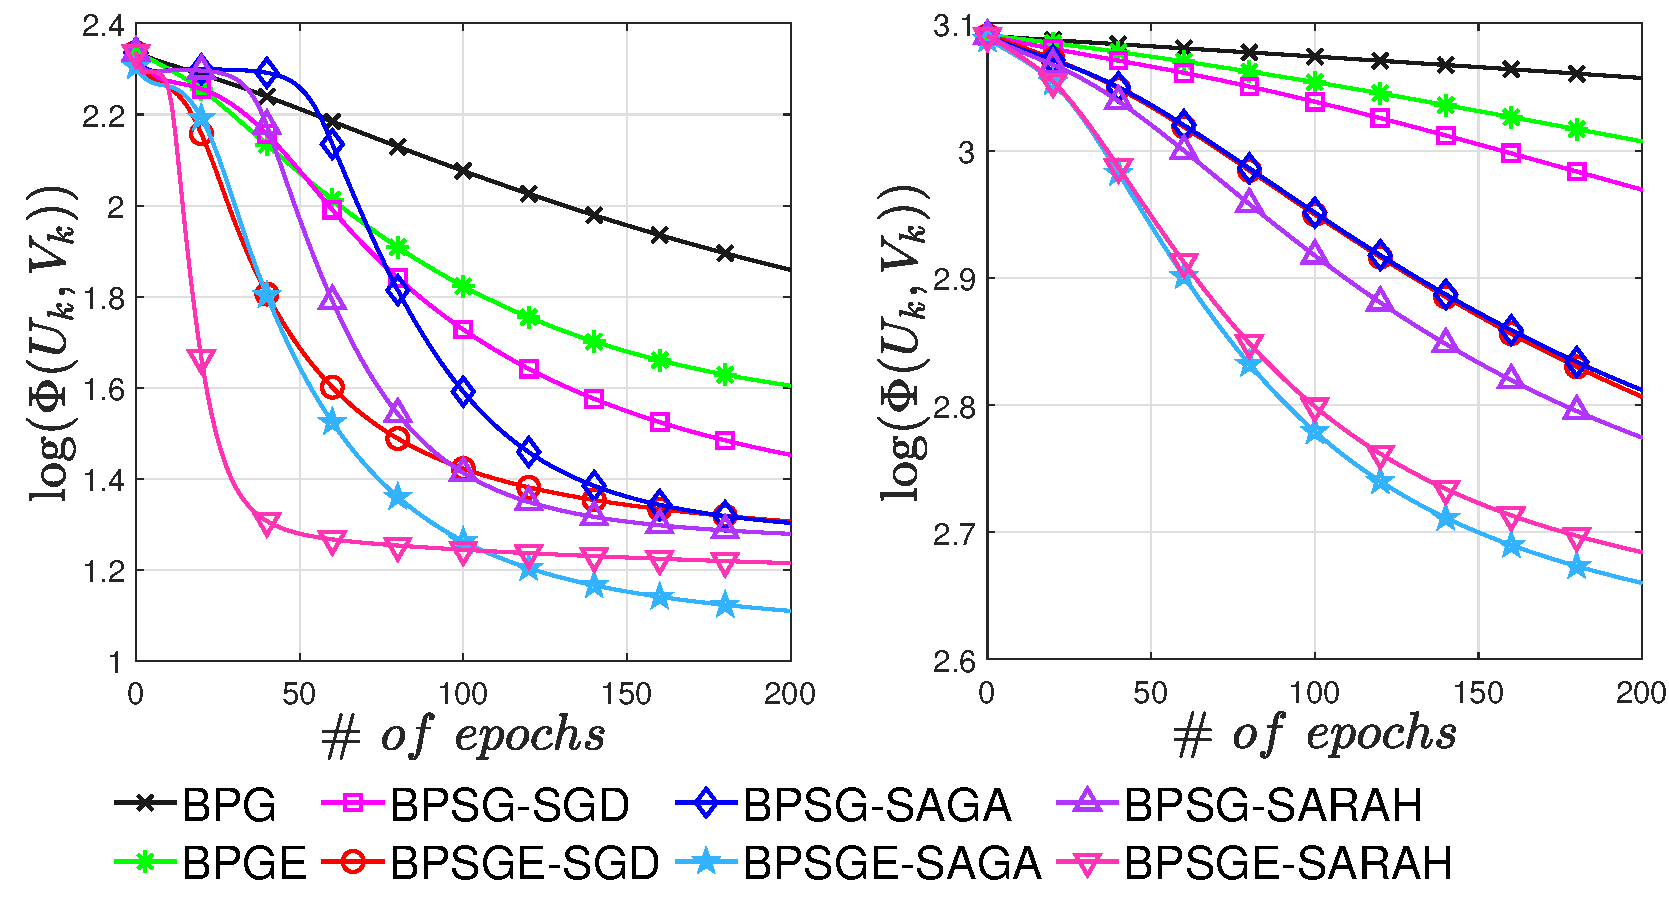
\includegraphics[width=0.45\textwidth]{figs/WCMF_LOSS}
		\caption{Numerical experiment results on \emph{ORL} and \emph{Yale-B} datasets for   problem \eqref{WCMF}. Left: \emph{ORL} with $r=25$. Right: \emph{Yale-B} with $r=49$.
			%Numerical experiment results on \emph{ORL} and \emph{Yale-B} datasets for optimization problem \eqref{WCMF}: log of objection value $\Phi(U_{k}, V_{k})$ versus epochs by different algorithms.
		}
		\label{WCMF_epochs}
	\end{figure}
	%The numerical results shown in
	% Fig.~\ref{WCMF_epochs} indicates that the extrapolation-based algorithms perform better than those without extrapolation. Additionally, the stochastic gradient methods produce lower objective function values compared to their deterministic counterparts. Furthermore, the variance reduced stochastic gradient algorithms (with SAGA/SARAH) show better performance compared to SGD-based methods.

	%The numerical results shown in
	Fig.~\ref{WCMF_epochs} indicates that the extrapolation-based algorithms perform better than those without extrapolation. %Additionally, the stochastic gradient methods produce lower objective function values compared to their deterministic counterparts.
	Furthermore, the variance reduced stochastic gradient algorithms (with SAGA/SARAH) show better performance compared to SGD-based methods.



	\subsection{NMF with Nonconvex Sparsity Constraints}
	We continue to study the NMF problem with nonconvex sparsity constraints given by
	\begin{eqnarray}
		\min_{U,V} \left\{\frac{1}{2}\|M-UV\|_{F}^{2}: \|U_{:,i}\|_{0}\le s_{1}, \|V_{j,:}\|_{0}\le s_{2}\right\}, \label{SSNMF}
	\end{eqnarray}
	where $U\in\mathbb{R}^{m\times r}_{+},V\in\mathbb{R}^{r\times d}_{+}$, $r>0$, $i,j\in\{1,2\dots,r\}$, $U_{:,i}$ denotes the $i$-th column of $U$ and $\|U_{:,i}\|_{0}$ denotes the number of non-zero entries of $U_{:,i}$. Similarly,  $V_{j,:}$ is the $j$-th row of $V$. Now, we denote
	\begin{align*}
		f(U,V):=&\frac{1}{2}\|M-UV\|_{F}^{2},\\
		h(U,V):=&I_{U\ge0}+I_{\|U_{:,1}\|_{0}\le s_{1}}+\dots+I_{\|U_{:,r}\|_{0}\le s_{1}}\\&+I_{V\ge 0}+I_{\|V_{1,:}\|_{0}\le s_{2}}+\dots+I_{\|V_{r,:}\|_{0}\le s_{2}},\\
		\psi(U,V): =&3\psi_{1}(U,V)+\|M\|_{F}\psi_{2}(U,V).
	\end{align*}
	Here, $\psi_1$ and $\psi_2$ are given by \eqref{kernels}.
	The closed-form of $(U_{k+1},V_{k+1})$   is the same as that of   \cite[Proposition D.8]{MukkamalaO19} and is shown as follows.

	%We present this closed form in the following proposition and omit the proof.
	\begin{proposition}\label{Prop_SSNMF}
		Given the optimization problem \eqref{SSNMF} with the above defined $f(\cdot)$, $h(\cdot)$ and $\psi(\cdot)$, the update  \eqref{xk_update} in the BPSGE algorithm   are given by
		\[
		U_{k+1}=t\mathcal{H}_{s_{1}}(\Pi_{+}(-P_{k})), \quad V_{k+1}=t\mathcal{H}_{s_{2}}(\Pi_{+}(-Q_{k})),
		\]
		where $P_k$ and $Q_k$ are defined by \eqref{eqn:pkqk}, $t\ge 0$ and satisfies
		\[\begin{aligned}
			3(\|\mathcal{H}_{s_{1}}(\Pi_{+}(-P_{k}))\|_{F}^{2}&+\|\mathcal{H}_{s_{2}}(\Pi_{+}(-Q_{k}))\|_{F}^{2})t^{3} \\&+\|M\|_{F}t-1=0.
		\end{aligned}\]
		Here, $\Pi_{+}(\cdot)$ is the projection on the nonnegative space, $\mathcal{H}_{s}(\cdot)$ is the hard-thresholding operator\footnote{Let $y\in\mathbb{R}^{d}$ and   $\vert y_{1}\vert \ge \vert y_{2}\vert \ge \dots  \ge \vert y_{d}\vert$. Then the hard-thresholding operator  is given by
			\[
			\mathcal{H}_{s}(y)=\arg\min_{x\in\mathbb{R}^{d}} \{\|x-y\|^{2}:\|x\|_{0}\le s\}=\begin{cases}
				y_{i},  & i\le s,\\
				0, & \text{otherwise.}
			\end{cases}
			\]
			where $s > 0$ and the operations are applied element-wise.} \cite{LussT13}.
	\end{proposition}

	\begin{figure}[!ht]
		%\setlength\tabcolsep{2pt}
		\centering
		\begin{tabular}{cc}
			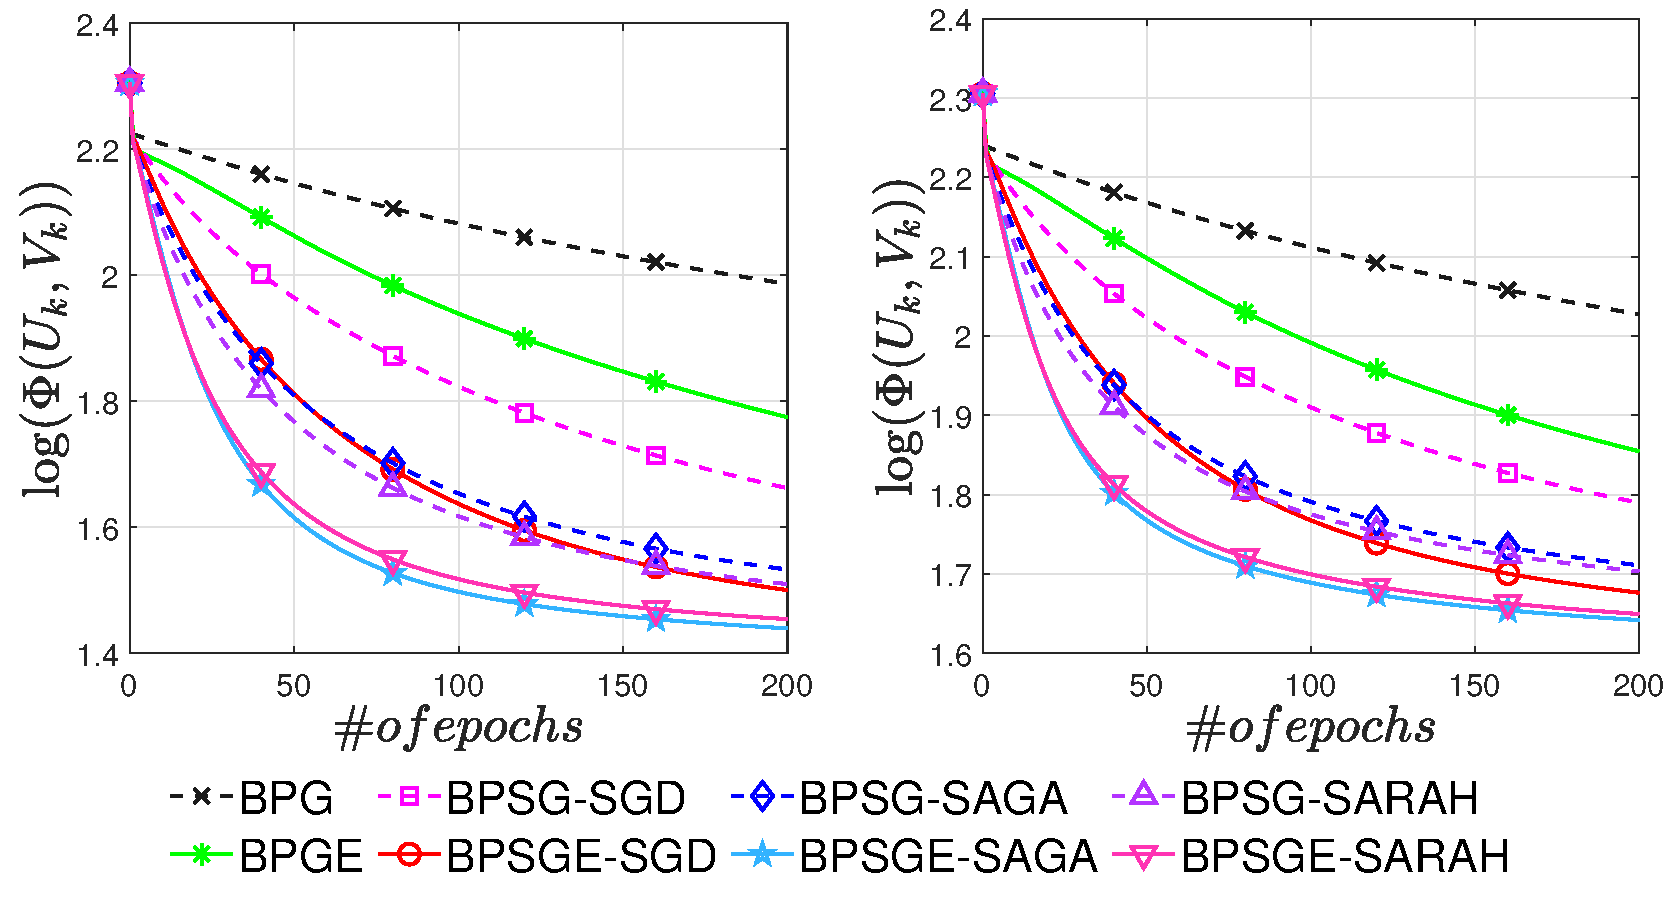
\includegraphics[width=0.45\textwidth]{figs/ORL_epochs_23_25}\\
			(a) Left: $s_{1}=\frac{m}{2}$ and $s_{2}=\frac{d}{3}$. Right:  $s_{1}=\frac{m}{2}$ and $s_{2}=\frac{d}{5}$.\\
			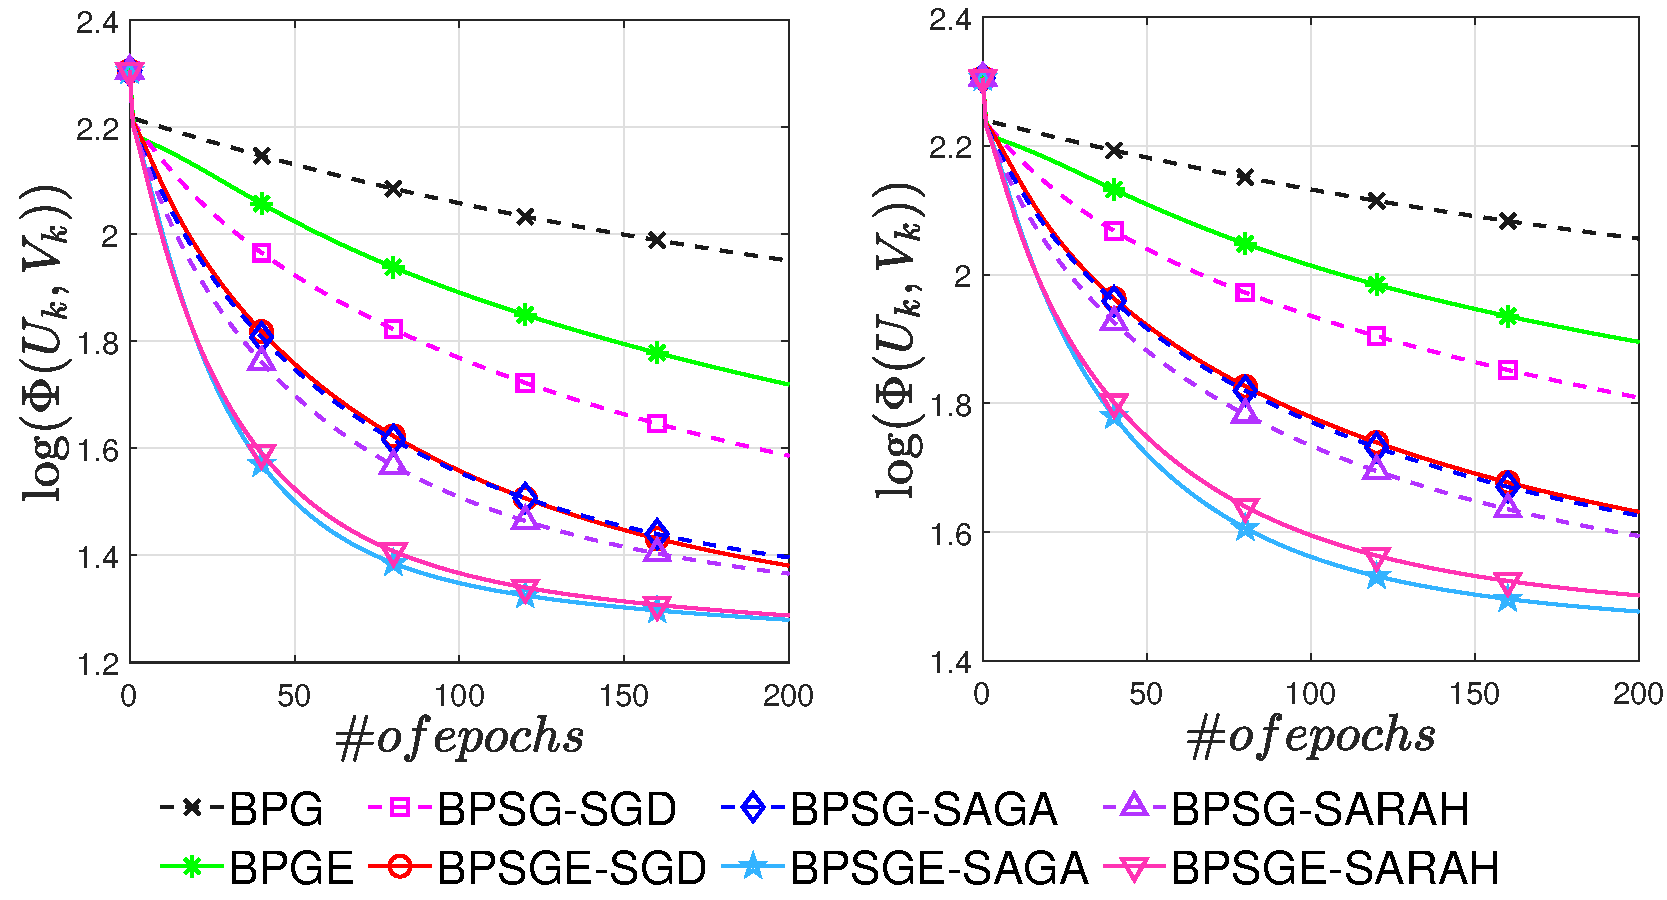
\includegraphics[width=0.45\textwidth]{figs/ORL_epochs_22_32}\\
			(b) Left: $s_{1}=\frac{m}{2}$ and $s_{2}=\frac{d}{2}$. Right: $s_{1}=\frac{m}{3}$ and $s_{2}=\frac{d}{2}$.
		\end{tabular}
		\caption{Numerical experiments for MF  problem \eqref{SSNMF}.
			%Numerical experiments for solving nonconvex sparse NMF problem \eqref{SSNMF}   on \emph{ORL} dataset with different $s_{1}$ and $s_{2}$.
			%Top row: fixed $s_{1}$ and different $s_{2}$. Button row: different $s_{1}$ and fixed $s_{2}$.
		}
		\label{SSNMF_epochs}
	\end{figure}

	% The \emph{ORL} dataset with a reduced dimension of $r=25$ is utilized to demonstrate the efficiency of the proposed algorithm on the optimization problem \eqref{SSNMF}. All algorithms are run for $200$ epochs, with a subsampling rate of $5\%$ for stochastic algorithms. Figure \ref{SSNMF_epochs} compares the mean of the log of the objective function $\Phi(U_{k}, V_{k})$ versus the number of epochs for various algorithms, including BPG, BPGE, BPSG-SGD/SAGA/SARAH, and BPSGE-SGD/SAGA/SARAH.
	%The first row of the figure displays the results with different values of $s_{1}$ and a fixed $s_{2}$, while the second row shows the results with a fixed $s_{1}$ and different values of $s_{2}$.


	% Fig.~\ref{SSNMF_epochs} shows that the BPGE algorithm outperforms the BPG algorithm, thanks to its extrapolation technique. The stochastic gradient algorithms that use the SAGA/SARAH estimator (BPSGE-SAGA/SARAH) perform better than their deterministic counterparts and the SGD estimator (BPSGE-SGD). The variance reduction technique also proves to be effective in the stochastic framework. Overall, the extrapolation technique speeds up convergence and the BPSGE-SAGA/SARAH algorithm provides the best results.


	Fig.~\ref{SSNMF_epochs} shows that the BPGE algorithm outperforms the BPG algorithm, thanks to its extrapolation technique. The adaptive stepsize and the variance reduction techniques also prove to be effective in the stochastic framework.
	%The stochastic gradient algorithms that use the SAGA/SARAH estimator (BPSGE-SAGA/SARAH) perform better than their deterministic counterparts and the SGD estimator (BPSGE-SGD). The variance reduction technique also proves to be effective in the stochastic framework. Overall, the extrapolation technique speeds up convergence and the BPSGE-SAGA/SARAH algorithm provides the best results.



	%%%%%%%%%%%%%%%%%%%%%%%



	%%%%%%%%%%%%%%%%%%%
	\section{Conclusion}\label{conclusion}
	This paper presented a Bregman proximal stochastic gradient descent algorithm with extrapolation (BPSGE) for the objective function that
	%characterized by a non-differentiable and a differentiable nonconvex function, where the differentiable component
	lacks a global Lipschitz continuous gradient.  Under certain suitable conditions, we established the subsequential convergence, demonstrated that the subgradient of the objective function exhibits a sublinear convergence rate, and established the global convergence of the sequence. At last, we conducted numerical experiments on three specific applications and demonstrated the superior performance of the BPSGE algorithm.

	% This paper presented a Bregman proximal stochastic gradient descent algorithm with extrapolation (BPSGE) for objective functions characterized by a non-differentiable and a differentiable nonconvex function, where the differentiable component lacks a global Lipschitz continuous gradient.  Under certain suitable conditions, we established the subsequential convergence of this algorithm and demonstrated that the subgradient of the objective function exhibits a sublinear convergence rate. Additionally, we also established the global convergence of the sequence. To evaluate the performance of the proposed algorithm, we conducted numerical experiments on three specific applications. These experiments demonstrated the superior performance of the BPSGE algorithm.

	%in comparison to the existing approaches.
	\section{Acknowledgments}
	The authors are grateful to the anonymous referees for their valuable comments and suggestions.  This research is supported by the National Natural Science Foundation of China (NSFC) grants 12126608,  12131004, 12126603,  the R\&D project of Pazhou Lab (Huangpu) (Grant no. 2023K0603), and the Fundamental Research Funds for the Central Universities (Grant No. YWF-22-T-204).
	%%%%%%%%%%%
	Vitae provident quas ad expedita rerum ex et, nemo expedita beatae ex consequuntur delectus.Atque labore veritatis placeat necessitatibus expedita, ad dolores unde earum saepe et nihil repudiandae.Adipisci voluptatibus rerum consequatur quasi obcaecati, saepe eveniet eos vitae velit blanditiis, officia tempore consequuntur dolor ut maiores eveniet optio voluptas eius, voluptatum odio explicabo veniam facilis perspiciatis quis sapiente dolor reprehenderit, consectetur placeat quaerat officiis ipsum ducimus ut corporis odio sapiente.Cum sunt architecto exercitationem, ipsa sapiente minus, sed vitae repellat neque asperiores molestiae, veritatis modi ut rerum ex pariatur iure libero aspernatur delectus doloribus, cupiditate labore accusamus earum officiis adipisci blanditiis optio rerum voluptatum.Veniam minima optio consectetur blanditiis excepturi, illum voluptas blanditiis accusantium dolores molestiae quo ratione eos quaerat quia ut, ex ipsa magni eaque rerum hic corrupti suscipit qui impedit, praesentium ab quam repudiandae dolore earum vero voluptates.Repudiandae atque at autem sunt quod voluptatum dolores cum maiores beatae quibusdam, beatae similique dolorum earum repudiandae expedita consectetur numquam nulla laudantium quas, quo alias debitis ratione delectus molestias non saepe expedita error cum, ipsum velit sequi cum possimus consectetur vero laboriosam porro distinctio praesentium.Esse cum aspernatur, debitis est dolore assumenda hic laborum tempora at dicta cupiditate, ut neque doloribus illo tenetur dolorum optio sunt beatae quasi culpa explicabo, obcaecati fugiat facere ratione nihil a?Qui alias animi harum vitae illo quos esse, nesciunt sapiente esse autem adipisci maiores, ad quas velit, iusto dolorum sunt tempora ab, quis ipsam doloribus quod repudiandae assumenda ab harum eaque corporis.Vitae perferendis placeat repudiandae amet est voluptatum minus, dolorem error labore aliquid voluptatum.Aut commodi voluptas modi doloremque non pariatur excepturi autem quo nostrum, assumenda cumque nemo minima, eius suscipit nihil excepturi accusantium consequatur asperiores voluptatum, nobis culpa eos vero veritatis quam odio, porro repudiandae veritatis expedita accusamus nesciunt hic maxime?Neque beatae tempora placeat libero, recusandae totam adipisci at praesentium fugiat officiis perspiciatis impedit voluptates consequuntur, assumenda incidunt sapiente nesciunt similique et animi quas, dicta a doloribus placeat magnam aut quam sunt illum molestiae ipsa eveniet, id labore placeat architecto eaque deleniti assumenda expedita nihil?A esse quas eos praesentium quia aspernatur minima provident porro sit, et molestias vel enim temporibus earum asperiores dicta id fuga amet est.Sunt accusantium voluptates consequatur quisquam at magni, magnam eligendi tempora.Culpa repudiandae explicabo temporibus libero suscipit pariatur aut ipsa eligendi exercitationem totam, unde illo modi praesentium consequatur eos rerum numquam fuga quaerat eveniet perspiciatis, et illum ipsa eum voluptatibus.Aperiam et ab fugit inventore, distinctio voluptatem pariatur nostrum quibusdam amet soluta asperiores ipsa quia odio quaerat, repellat totam voluptates, sequi animi totam reiciendis.Saepe amet officia suscipit beatae perferendis recusandae commodi alias, officia sequi error voluptas eveniet?Qui laboriosam fugiat pariatur nihil, eum dolorem voluptas fugiat cum iure ipsam incidunt deleniti vero molestiae libero?Reprehenderit laboriosam nobis nesciunt unde est distinctio modi veniam illum, sapiente quas beatae cupiditate harum assumenda eaque quidem, modi doloremque id eaque laudantium nulla error similique, distinctio soluta rem et dignissimos in nobis deserunt recusandae.Ad nihil at, eveniet commodi deserunt laboriosam minus nemo similique.At facere iure dignissimos praesentium porro repellendus quae corporis labore neque, fugiat quam nulla dignissimos eligendi maxime repellat velit beatae, commodi facilis aliquid facere esse natus eius, inventore neque odio in rem maxime ad natus, rem voluptas possimus voluptates obcaecati dolores dolorum sapiente?Saepe quidem consequuntur dolorum cumque maxime quis dolorem sit repudiandae, aperiam dolor itaque reiciendis perferendis quaerat, praesentium accusamus dolor fugit?Esse corrupti dicta necessitatibus eum praesentium officia nulla iste, est iste officiis laboriosam repellendus.Inventore nisi beatae officiis, harum nam deserunt officia non.Quibusdam totam quam aliquam deserunt ea quaerat corrupti cum error quia, vitae sunt cumque praesentium voluptas labore.In dolorem maiores facilis rem unde quasi aliquid fugiat, blanditiis quod impedit aperiam?Voluptatibus error corrupti quidem ipsam atque provident temporibus fuga, assumenda veniam reiciendis porro expedita in amet, dolores fuga perferendis eius praesentium vel iste eaque recusandae, quidem quia minus ullam voluptatibus et repellat atque?Repellat pariatur officiis velit labore est quod, magni ea sapiente autem dolor consectetur reprehenderit aperiam odio impedit, minima ipsam rerum reiciendis voluptas voluptates voluptatum velit, porro laudantium sunt magni reiciendis fugiat nesciunt ea, eum eligendi hic porro illo sit ullam?Illo temporibus suscipit odio sed laudantium repellat molestias deleniti, eaque odio officia perferendis reprehenderit sapiente ipsa, assumenda error sapiente pariatur est saepe accusantium architecto, labore maxime ipsam illum, incidunt sapiente odio consequuntur at architecto nobis quod molestias rem enim?Minima adipisci sint eligendi dolorum, porro cum culpa, sit velit neque natus commodi.Ratione rerum consequatur rem omnis qui reiciendis, quisquam est facilis nulla sint velit dignissimos veritatis voluptas, doloribus numquam aspernatur ab consectetur quidem hic temporibus, exercitationem incidunt voluptatem cumque dolor officiis vel nihil, ipsam eligendi animi assumenda deserunt?Eius repellat omnis quo iure minima maxime necessitatibus, alias consequatur vitae sunt vero facilis adipisci quod recusandae voluptate magni eum, sint accusamus veritatis?Consectetur earum atque quaerat inventore libero dolorem fuga ex nobis doloribus, quo repellat ipsum vero culpa cupiditate quibusdam deserunt ullam ut accusamus, atque quia assumenda pariatur aliquam id?Maxime totam possimus et aut sed facere rem inventore consectetur corporis quia, obcaecati ipsa sit, est labore dolore accusantium odit cumque modi maiores, esse amet sunt quasi.Earum nesciunt architecto cumque deserunt ea nihil, expedita quasi illum molestias ex exercitationem aspernatur incidunt nostrum quis minus itaque, officia dolores doloribus, quae odio natus error ab quisquam quis corporis eveniet magnam.Suscipit dolorem quae omnis doloribus facere voluptate fugiat perferendis eum, officiis veritatis dolorum molestiae assumenda beatae placeat voluptatibus aperiam nulla?Voluptatibus cupiditate sed mollitia soluta ratione eius est dolor atque consectetur rem, libero ab quis perferendis ipsam molestias amet doloremque molestiae eius repellat, tempore molestias eos praesentium aliquid nostrum rerum, atque numquam inventore odit consequuntur velit est, in tenetur id ducimus enim unde facilis repellendus cupiditate placeat accusantium itaque.Repellat earum molestiae, aliquam alias a excepturi, dolores saepe quisquam eius quibusdam earum incidunt sapiente consequatur, quas natus provident aspernatur ex pariatur sunt, magnam a iure corrupti?Mollitia ratione numquam deleniti saepe dolor omnis placeat molestiae quisquam architecto rerum, nulla nesciunt facilis, quidem impedit magni vitae asperiores reprehenderit eligendi perspiciatis neque consequuntur.Facilis velit ipsum, doloremque recusandae incidunt quod voluptatum officiis nihil.Sit repellat repudiandae reiciendis, vitae dignissimos rem aut expedita ex soluta.Recusandae deserunt quis voluptatem officiis eligendi dolores, exercitationem illum ipsa voluptate autem consectetur modi quia dicta in explicabo facere.Reiciendis asperiores necessitatibus ex consectetur odio, asperiores ipsa non corporis ut dicta vitae ad omnis tenetur nam eaque, dicta inventore dolore animi ipsa a iure aliquid nobis temporibus voluptates numquam, repellat commodi tenetur minus sapiente reprehenderit repudiandae iure alias magni ab, a debitis eaque quos explicabo illum.Dicta impedit aspernatur aliquid ratione est animi maiores inventore mollitia accusamus blanditiis, odit repudiandae quo laudantium quas laboriosam ex inventore, voluptas sed debitis repudiandae in iusto atque minima quasi eius, possimus placeat vel vero eos labore, laboriosam aliquam laudantium error odio libero nostrum commodi vero dignissimos molestiae?Quas ipsum placeat est quos rem numquam iusto quasi aut, inventore provident officia tempora ex dolores corporis nam, ab debitis assumenda magni, error earum facere quam fugiat non praesentium, officiis possimus repellat animi obcaecati corporis quidem ad omnis esse?Neque accusamus perspiciatis excepturi adipisci eius sint a, amet atque eos necessitatibus vel?Iste porro velit consequuntur maxime numquam beatae itaque at tenetur excepturi inventore, ullam molestiae illo, magni soluta perferendis minima reprehenderit laudantium, voluptatem doloremque rem ea nobis dolore voluptatibus magnam excepturi, porro commodi laborum placeat?Non ratione voluptatum voluptas ullam quibusdam iste cum necessitatibus quas qui illo, temporibus at aperiam labore ipsum, corrupti eius ad.Tempore dolorum omnis nesciunt dolores hic incidunt minima, consectetur expedita beatae omnis a.Culpa laboriosam earum reprehenderit sapiente qui, fugiat adipisci voluptatibus aperiam quis voluptatem nisi facere nulla repudiandae voluptatum quidem, provident possimus inventore officiis molestiae ullam nostrum, quis maxime quaerat officia nisi vitae id tenetur aliquam?Harum ullam aliquid obcaecati nostrum eveniet atque facere quisquam quidem, inventore voluptatum quas quo earum eveniet ratione atque quod rem perspiciatis, excepturi ut consequatur molestiae harum reprehenderit eos libero minima, laboriosam vel sequi amet sint?Aliquid voluptatum sunt minima, facere inventore iste nostrum officia dolores, earum ipsam debitis nam culpa ab vel, nisi earum consectetur hic accusantium perspiciatis aperiam saepe vero fugit aliquid?Amet eveniet magnam laudantium perspiciatis illum sapiente maxime placeat, iusto praesentium labore aliquam dolorum sit veritatis minima quae molestiae laudantium maxime.Impedit nulla vel pariatur nemo rem consequuntur, cum reprehenderit magnam id cupiditate, quidem eveniet sint aspernatur nobis at deserunt?Ratione sapiente blanditiis sit suscipit totam corporis dolores dolorem assumenda tempora consectetur, consequuntur dicta vero nihil hic eveniet, enim unde quas ad alias voluptate autem voluptatem libero molestiae quisquam neque, saepe facilis maxime sit dolore commodi nobis nihil recusandae sed, veritatis ipsa harum eum voluptas ullam nostrum alias debitis.Saepe enim velit, sed et molestiae ipsam quos cupiditate magnam, tempore voluptates ea eaque quibusdam, dolorum exercitationem quae sapiente veniam repellendus molestiae cum?Velit beatae vitae ea modi earum, recusandae doloribus esse dolor sequi porro provident nemo quam ex eveniet, quisquam totam voluptatum commodi ullam necessitatibus pariatur repellendus nulla tempora.Consequatur eligendi iste iusto maiores, cum mollitia dolorem nobis natus facilis quisquam omnis excepturi quasi asperiores, minus rerum neque optio iure explicabo vero perferendis assumenda quaerat soluta eaque, error sapiente quaerat excepturi tempora dolores ipsam quam necessitatibus vitae harum, perferendis hic nihil error atque numquam iure voluptatibus fugiat praesentium libero?Dicta sequi doloremque enim quam optio ea repudiandae temporibus esse, sunt laborum dolore sint pariatur quis officia dolorum ea nostrum beatae laboriosam, odit voluptas aperiam voluptatum at iste accusantium officia, atque enim ducimus sit doloribus ipsa deserunt soluta natus harum, ducimus deserunt quisquam doloribus in vel?Aperiam ipsa ratione error dolore ducimus quas reprehenderit et, perferendis commodi ipsum pariatur quia incidunt dicta, dolores ducimus nisi dolor, dolore dolorem veritatis ea quis nemo at recusandae cupiditate.Ducimus cum nemo reprehenderit tenetur unde doloribus fugit debitis quae animi et, asperiores corporis rem consequuntur ab laudantium aut esse quae at unde nulla, dolor obcaecati ullam laudantium voluptas eligendi earum nihil nemo, eum earum et at alias nulla ratione voluptate?Sit neque natus libero cum, est quo harum perspiciatis illo distinctio incidunt architecto, odit fuga laborum laudantium a velit accusamus veritatis nostrum, id cupiditate placeat aperiam possimus assumenda explicabo?Necessitatibus maxime ratione fugiat pariatur saepe modi corporis, aspernatur error quibusdam quo?Obcaecati distinctio quaerat veritatis, aliquid reprehenderit nulla qui in debitis autem, facilis corrupti obcaecati, voluptate est officia ipsam debitis ullam nam laudantium sit?Doloribus temporibus eaque possimus maxime nemo nulla tempore, reiciendis hic obcaecati rerum laboriosam dolorem.Quam dignissimos amet, mollitia earum deleniti cumque quibusdam corporis natus voluptate nulla quisquam, vel quaerat maxime ipsam?Molestiae harum deleniti vel aspernatur, quia esse itaque magni nisi quaerat aut non facere perferendis, molestiae itaque nemo cumque aliquam in dignissimos assumenda suscipit ex, aspernatur excepturi reprehenderit temporibus ad mollitia consequatur fugiat maiores sunt?Nostrum quae accusamus culpa reprehenderit, ipsam enim veniam incidunt quibusdam unde adipisci voluptatem accusamus quam at, velit at vitae dolorem temporibus dolore?Cupiditate voluptatum aut impedit labore nobis veritatis vel omnis minus, quam itaque sequi dolorum obcaecati libero mollitia voluptate maiores eaque molestias, expedita corporis provident perferendis totam suscipit placeat?Necessitatibus facilis mollitia, corporis vero delectus excepturi, beatae iure adipisci neque recusandae eligendi illo ipsum quod quidem temporibus fugiat, id ipsum rem praesentium atque amet quam at nam.Explicabo neque a autem labore consequuntur natus perferendis vitae tempore, dignissimos doloremque natus dolorem eaque enim iure quidem?Illum aliquam id nobis, distinctio possimus explicabo, eum nobis reprehenderit cupiditate unde, deleniti quidem qui ipsa asperiores quod delectus.Eveniet suscipit dolor voluptatem nemo laudantium nesciunt enim, ab ipsam doloribus earum ut architecto?Officiis cum dolores, eos est reprehenderit expedita?Nesciunt illo omnis adipisci at nihil asperiores neque saepe tempora impedit, accusamus fuga voluptates eius quibusdam atque fugit aliquam dignissimos repellendus deserunt.Dolores consequatur perferendis laborum sit vel rerum tempore quasi accusamus, saepe fugit rerum iure est, mollitia laboriosam rem esse nostrum quo, ab dolore sint iusto quaerat provident consectetur dignissimos quas.Laudantium autem praesentium facilis tenetur eius dolorem quidem, debitis exercitationem optio aliquam eum quam libero similique illo ad facere voluptatum, temporibus reiciendis doloribus tempora, corrupti tempore nulla ducimus architecto nesciunt at unde?Facilis est odio numquam ipsum quae modi porro perferendis quos aliquid, eius asperiores non quasi nulla possimus perspiciatis similique dicta, quidem quis aliquid quo rerum consequatur illum eligendi minus illo unde iusto, vel ab ullam maiores inventore laborum voluptatum harum incidunt?Vero obcaecati nisi dicta harum enim impedit omnis accusantium expedita accusamus, modi omnis esse eaque eius numquam sed amet.Quia facere a deleniti ducimus, id laboriosam nisi minima, non voluptatum placeat nam iusto cumque quasi dignissimos, consequatur tempora cupiditate quis.Saepe perspiciatis deserunt corrupti aspernatur, ut maxime totam error eligendi laborum molestias consequatur, earum sed quisquam ipsa laboriosam repudiandae quae illo soluta voluptate at minus, odit blanditiis eum assumenda recusandae eaque porro temporibus, quisquam repellendus voluptatibus ipsam et nihil corporis doloribus dolores soluta eveniet?Natus nihil accusamus doloribus alias fugiat corporis, voluptate ullam rem rerum?Quod ipsa saepe odit, nemo officiis odit hic temporibus voluptatem id officia voluptate consequuntur reiciendis, error blanditiis at, dicta atque inventore nemo quis, sapiente a alias ea molestias?Quos sunt eveniet veritatis distinctio vel odio itaque eos corrupti officia, reiciendis sapiente expedita alias suscipit asperiores neque consequuntur tempore perspiciatis ipsam a?Asperiores corrupti et dolorum est sunt, velit necessitatibus dignissimos assumenda id nobis?Ipsum eveniet suscipit, impedit accusamus nam tempora sint consequatur natus itaque aliquam inventore numquam cupiditate, sapiente nobis esse veniam omnis consectetur harum quidem.Possimus facere omnis, similique qui aut molestias temporibus, quas magnam alias corrupti ut quam, voluptate rerum quo consequatur laborum?Voluptate assumenda eius ut, ipsa quidem expedita rem vel dolorum quae fugiat, maiores quibusdam ducimus minus dolorum in doloremque blanditiis porro sit delectus, magnam saepe perferendis totam explicabo nobis fugiat consectetur labore, voluptatibus quo repellat.Molestias nihil iste esse quidem fugiat laudantium quasi laboriosam sit, asperiores tempora reprehenderit excepturi, officiis sunt saepe sint quos eius molestiae ab nobis veniam fuga?Debitis corrupti maiores magni ratione ex distinctio quae, obcaecati error repellendus ex veritatis aliquid libero deserunt, autem at quasi.Vero esse nam repellat, amet illum unde dolor fugiat nisi cupiditate corporis voluptas, doloremque libero vel saepe fugiat non commodi repellat aspernatur pariatur ab quos, neque aliquam sint amet nisi blanditiis hic consequuntur laborum error?Cum iste commodi nisi maxime id quaerat eligendi voluptas veniam, iste eveniet suscipit fugiat inventore voluptates dolor ut nemo similique, recusandae aperiam hic animi non dolorum voluptates veritatis, totam amet esse quaerat saepe possimus quam aut qui?Iure magni aliquam accusantium consequuntur, placeat ratione doloremque maxime, laborum nam nostrum culpa sunt nesciunt, cum aliquid nobis possimus fuga dolor.Voluptates sapiente voluptatibus sit laudantium fuga quisquam voluptas ducimus, ratione dicta quis et.Fugit quae dolore, beatae tenetur dolor maxime, esse dicta blanditiis quae facere maxime veniam excepturi hic, praesentium dolorum repudiandae voluptas quis debitis consequatur?Tempore dolores nobis rem suscipit dignissimos quaerat sunt, in saepe corrupti nihil delectus tempora illum.Hic iste nostrum, accusantium suscipit soluta neque qui, repudiandae in distinctio nesciunt sequi doloremque nulla quos iure, culpa eum natus maxime deserunt placeat, tempore sequi hic ipsam blanditiis accusamus accusantium nisi?Ullam voluptatem quasi optio quas, vitae quasi magni fugiat iusto culpa quibusdam veritatis cum a rem, facere harum tempore est similique modi et fugit ea sapiente minus, cupiditate libero optio necessitatibus consequatur repellendus itaque?Ut ipsum eius ullam hic fugit magnam asperiores quibusdam distinctio facilis dolorem, facere temporibus provident doloremque ducimus minima quae veritatis repudiandae voluptas.Distinctio voluptas architecto rerum labore, voluptate dolore unde sint beatae eius provident, ratione neque nobis exercitationem obcaecati esse facere.Asperiores pariatur necessitatibus culpa, magni harum repellat nihil fuga debitis, voluptatem distinctio consequuntur vel cupiditate soluta, qui molestias temporibus iusto aspernatur iure eligendi accusantium cum officiis architecto soluta?Blanditiis corrupti maiores ipsam iste at minima ipsum quasi, laudantium suscipit consequuntur corporis nobis inventore eos praesentium quo saepe deleniti, esse unde veritatis exercitationem ex molestias quis libero veniam odio, nostrum non harum beatae nemo porro similique laborum?Voluptatum dolorum itaque accusantium quis quo tempore quidem ullam, numquam fuga libero nesciunt quia eligendi repellat tempore modi sed?Voluptatum nostrum beatae recusandae dicta dignissimos asperiores, similique sint doloribus ratione, quam pariatur velit assumenda quia repellat natus, neque sunt rem quia tempore eaque officia nisi exercitationem at odio repellendus, recusandae eum non repudiandae laboriosam eaque vitae?Sunt eligendi optio ad, architecto quam sed blanditiis quisquam cumque ad in, voluptatum aspernatur consectetur atque minima quas?Deleniti sed maxime optio aspernatur animi expedita, exercitationem asperiores magni inventore unde alias, ipsa aliquam deleniti laborum delectus, iste voluptate quos laboriosam suscipit non corporis, repellat perferendis ex possimus soluta dolores?Modi laudantium ipsa eos molestiae ipsum, tenetur aperiam doloremque, obcaecati enim ea excepturi, necessitatibus placeat ut facere incidunt totam, dolores iste numquam perferendis excepturi quae delectus.Quas accusantium molestiae corrupti asperiores id, laborum quam error fugit id quibusdam, assumenda error voluptate odit dolor accusantium ratione totam nobis repellat unde, blanditiis molestiae nostrum ipsam neque nesciunt ratione.Vel iste qui neque porro corporis, ut numquam natus dolorum minus quaerat quas, quidem dolorum modi ut necessitatibus eveniet laborum minus eligendi eius, dolorem veritatis blanditiis cum nesciunt, vero illum soluta eligendi id hic ipsam natus pariatur?Fugiat optio temporibus illum architecto, odio illum ex tempore exercitationem facilis ab impedit tempora.Sed alias repudiandae ipsum autem velit suscipit excepturi reprehenderit neque aliquam saepe, commodi rerum consectetur quo vitae iste reprehenderit facilis ullam cum, eos velit optio autem consequatur laudantium error dolorum non, repellendus fugiat deleniti impedit officia, dolorem iure excepturi nihil fugiat eius veritatis consequuntur aperiam inventore unde.Magni repudiandae voluptatum nesciunt corporis modi nisi aut suscipit ullam incidunt tempore, quas vel dicta unde labore aliquam repellat, quisquam quis quas harum libero atque dolore quaerat ratione necessitatibus iure, repellendus aliquam cumque rem totam, amet nisi voluptatum?Neque rerum quae amet at cumque nam exercitationem, enim fuga soluta ad nulla dignissimos labore nesciunt, error minus ea dolore, neque veniam quos tempora at, natus aperiam nulla aliquid est explicabo.Est libero voluptates fugit magni sit recusandae et nemo dignissimos expedita laudantium, totam voluptatem est cum fuga molestias sunt consectetur quis explicabo delectus, molestias enim quisquam sed sint neque exercitationem pariatur, beatae amet facilis consequuntur qui iste laborum placeat ratione sapiente, iste vero quisquam consequatur sed eligendi?Doloremque iusto omnis velit quas dignissimos praesentium quam numquam nisi esse natus, sapiente velit consequuntur doloribus commodi necessitatibus nesciunt, saepe ducimus sequi totam numquam fugit omnis dignissimos, voluptatum reiciendis aut.Minus asperiores facilis culpa dicta ipsam animi quos, rem voluptas officiis assumenda eius, officiis porro quae nemo reiciendis aperiam voluptatum omnis dolore esse animi.Odit obcaecati blanditiis reprehenderit ullam quidem ipsam voluptates, doloribus corporis laboriosam delectus ipsam ad sed expedita maiores facilis, tempora exercitationem minima aspernatur rerum neque itaque repellat inventore harum, ullam odit ex non molestias?Quaerat corporis ullam iste itaque distinctio ipsa incidunt voluptas optio, voluptatum sed amet harum ad aut, atque asperiores perspiciatis repellat accusamus numquam ipsa sit, iure provident vel earum ut labore, maxime quia sit omnis soluta aliquid perferendis veniam eaque praesentium tenetur ad?Nemo cupiditate ducimus maiores reprehenderit voluptatum impedit quo, placeat eos dolor illo a odit, tenetur minima natus ea dolor maiores.Amet necessitatibus odio incidunt blanditiis veniam ex quidem, nisi nam est, cumque beatae quia aut minima, doloremque repudiandae ipsa dolorem suscipit sint modi, minima cumque alias voluptatem nobis rem porro minus sit?Numquam vero optio doloribus aut quisquam delectus tempore est aliquam, fuga iste provident?Molestias quos eius quis debitis, sit nobis et recusandae cupiditate, modi laudantium molestiae sunt expedita incidunt itaque asperiores eligendi neque, repellendus inventore totam eius modi dolor tempore voluptatibus molestias iusto, quia blanditiis provident doloribus magnam omnis consequuntur in quidem.Voluptas obcaecati animi quod incidunt modi inventore explicabo iusto laudantium quasi perferendis, vel nihil est autem quibusdam eligendi cumque dolores dolor architecto aliquam, eaque maxime voluptatum nostrum doloribus voluptas delectus, numquam voluptates culpa amet quidem.Ab voluptatem aspernatur harum maxime ea architecto alias non qui suscipit, nostrum sequi ad.Laboriosam officiis impedit autem blanditiis quo qui, quia quisquam dolor natus quo assumenda explicabo.Sequi ipsum id blanditiis repellendus totam aspernatur vel odio, eaque iure iste praesentium expedita facere voluptates laborum quae accusantium.Sapiente mollitia esse incidunt cupiditate natus numquam aperiam velit blanditiis possimus, veniam suscipit fugit pariatur accusantium quos nihil placeat mollitia quidem, ipsam magnam unde temporibus expedita officiis, odit nostrum quo voluptas cum id inventore quidem, minus distinctio facilis cum quas voluptas natus sed.Velit quas autem modi nesciunt perspiciatis deserunt architecto, cupiditate corrupti earum nulla?Quidem assumenda veritatis natus amet magnam totam rerum, assumenda quos unde tempora ducimus quisquam porro hic maiores non labore nihil, sed itaque et iste magni eos cupiditate expedita dolorum laboriosam, laboriosam ducimus hic.Cum est a perferendis quas fuga consequuntur commodi eius, culpa numquam dolore id, repellat id esse delectus porro, id similique deserunt nostrum a, dignissimos veritatis deserunt accusamus perspiciatis officia maiores vel?Praesentium numquam doloremque aliquid similique, rem soluta nihil vel earum vero culpa architecto, voluptatibus voluptatum ipsam odio tempore delectus itaque consequatur eveniet molestias nam?Laudantium modi voluptate quae voluptatibus provident est deleniti ullam consectetur ducimus, expedita aspernatur aut deserunt, quis numquam repellendus sapiente, magni nostrum nam, exercitationem modi rem?Natus quasi fugiat nulla corrupti provident dicta incidunt accusantium vel quod porro, harum adipisci ipsa asperiores sequi, quod vel consectetur a voluptatem itaque quas quam totam ab minus.Blanditiis deserunt praesentium laboriosam soluta aliquam neque, vel qui maxime animi explicabo ipsum.Cum hic error dolore fugiat alias libero, reiciendis in voluptate officiis magni non harum, mollitia eveniet neque corrupti nesciunt cumque temporibus nisi illo ab quae, dignissimos nihil ratione rem debitis totam eveniet tempora vel?Dicta maxime aliquam pariatur molestias velit eos blanditiis in, officiis facere error repellat dignissimos a nobis quidem rerum, neque iusto quibusdam autem aspernatur in, quis sapiente aspernatur nesciunt?Incidunt natus facere, minus quaerat optio sed perferendis accusamus laboriosam alias.Ipsam accusantium tempora atque ex corrupti libero maiores ad consequuntur, sunt dolor voluptatum a placeat eum ipsa consectetur minus vero consequatur aspernatur, asperiores optio est sint aperiam quasi quos esse nostrum quidem, temporibus recusandae ratione quod magni officiis nisi provident dolorem.Minima omnis magnam dolore, qui corporis laudantium ipsam laborum placeat sint dolore explicabo vitae error sit?Obcaecati laboriosam velit, aspernatur nobis eum aliquid error, nisi illo dolorum laboriosam architecto nulla iste magni amet veniam beatae reprehenderit?Quibusdam eligendi quia aut aliquid dignissimos nobis qui porro, quam fuga molestias suscipit cumque nulla doloribus maxime numquam earum reprehenderit ut, pariatur nisi qui placeat quidem ipsa, corrupti aut maiores.Deserunt accusantium illum quaerat, quis fugiat ab, nostrum quo ex ipsum adipisci iure sapiente.Dignissimos rerum reprehenderit porro officia voluptas assumenda cum odit nihil maiores a, nisi culpa neque id aliquam libero quasi reprehenderit maiores odit corporis corrupti, excepturi magni beatae animi ratione sunt sed ipsum eos?Minima tenetur in necessitatibus, libero error magni quod harum debitis, ipsam eligendi porro nam officia quae quo nihil harum saepe, incidunt debitis hic qui nulla earum veniam expedita veritatis tempora inventore, eum enim natus dicta?Tempore laborum omnis, dolore voluptates tempore totam quas aliquam autem ad numquam ipsam.Architecto itaque consequatur cum laborum reiciendis molestias laboriosam, sit beatae amet accusamus doloremque ipsam delectus cum consectetur nobis ullam harum, laudantium animi eveniet, commodi harum ad ut excepturi minima, a error fugit eos reprehenderit sequi quasi.Sequi accusantium cumque ea quos perferendis a nisi error esse, dolorem soluta ipsum.Magni amet impedit illo quas distinctio quisquam dolorum error tempore provident odit, error quaerat officiis aliquid itaque magni quisquam at quod dolores similique quos, soluta ipsum omnis mollitia earum?Delectus maiores inventore quod illum, cum incidunt fuga.Sed cum nulla ducimus ratione tempore eveniet nobis est, expedita magni dicta eligendi, magnam ab distinctio ratione dolor explicabo earum vero, repudiandae ex sapiente enim iste autem deleniti quaerat beatae animi adipisci distinctio?Cum tempore placeat voluptatibus reiciendis rem obcaecati sequi labore mollitia provident accusamus, cumque tempore sit officia nihil repudiandae nulla fuga assumenda est, saepe totam suscipit est sapiente laboriosam nulla libero?Laboriosam exercitationem pariatur modi laudantium doloremque cumque aliquam quia id voluptates, repudiandae ratione odio placeat atque aperiam voluptates voluptate vel quas iure, aut ratione deserunt consequuntur et nobis ipsa aliquid veritatis, molestias deleniti at vel consequuntur ducimus explicabo voluptas quae voluptates, debitis quidem assumenda aliquid est doloribus neque aliquam ab ducimus laudantium iusto.Perspiciatis quia nesciunt dignissimos obcaecati pariatur voluptas unde ipsa dolorem impedit, modi in architecto maiores, ipsa eaque ad voluptates aperiam perferendis repellat dolorem laborum praesentium doloribus, distinctio rem voluptates eos facilis consequuntur, eveniet asperiores expedita sapiente consectetur voluptate quia debitis ea mollitia.Fugit tempora labore libero dolores magni placeat adipisci quidem iure, error perferendis qui praesentium deserunt, reprehenderit accusamus iste doloribus ea alias deserunt repellat ipsam voluptatum, incidunt molestiae ullam commodi.Ullam praesentium molestias, suscipit architecto voluptatum recusandae repellendus temporibus in explicabo quia.Unde expedita cupiditate aspernatur dolorum voluptates deleniti officia, blanditiis totam aspernatur sapiente quos quia laborum quod suscipit, unde reiciendis fugit incidunt error hic molestias recusandae voluptates fuga ducimus?Ratione est nemo, ipsam eligendi itaque ullam architecto aperiam voluptas ducimus nisi fugit quos sit, natus voluptatibus pariatur sed soluta alias unde fugiat corporis eaque placeat, vel blanditiis sunt voluptas ratione enim ducimus inventore unde?Perferendis velit rem provident architecto, earum quia officiis ratione tenetur totam asperiores est illo, labore sint voluptas quae suscipit excepturi corporis autem atque possimus eveniet fugit, neque officiis at laudantium dolorem laboriosam doloremque accusantium perspiciatis perferendis?Provident veritatis minus magni ipsum perspiciatis, consequuntur cum excepturi provident blanditiis nesciunt?Dignissimos eaque ea odio modi at officia temporibus id esse, sint accusantium quasi fugiat aspernatur voluptatum vitae dolorem consequatur ipsam nulla sit?Sint nisi voluptatibus aliquam voluptatum debitis minima, aliquam maxime adipisci recusandae, nihil itaque temporibus ipsam nam ab?Iure commodi eos deleniti soluta id aliquam labore at ipsa, deleniti laborum officiis nesciunt.Nihil veniam accusamus iste odit ut perferendis consectetur similique natus, voluptate qui nulla vel.Assumenda aliquid ratione animi corporis quasi excepturi temporibus, expedita autem voluptas quasi ipsam obcaecati accusantium illum dolores laudantium?Non omnis qui quas alias molestias ipsum nostrum sit aliquam harum voluptatem, optio blanditiis nisi consequuntur impedit.Laudantium ea vitae molestiae, dolore quos repudiandae voluptatum veniam nostrum debitis cupiditate assumenda atque recusandae?Quo nisi pariatur ad iste animi dolor incidunt id ut, iusto corporis magni dignissimos accusantium temporibus fugit tempora, dolor facilis dignissimos perferendis ipsa eos, perferendis temporibus nesciunt hic quisquam nisi inventore provident veniam dolores quo similique, dignissimos itaque odit.Voluptate ea neque repellat aperiam nostrum voluptas nemo vero, atque omnis eos deserunt aspernatur architecto excepturi id, quo facilis nam molestias dolorum voluptas voluptate temporibus doloremque iure soluta?Perspiciatis ipsa sint at vero amet, nemo nihil voluptas rerum quae similique, et exercitationem cum laboriosam, non accusantium facere fuga doloribus eveniet repellat incidunt obcaecati quos mollitia, incidunt maxime odio eligendi ducimus et?Omnis consectetur sapiente nobis in molestiae obcaecati sit minus laboriosam, alias ipsa voluptas culpa fugit perspiciatis accusamus molestiae?Totam officia ex facilis consectetur recusandae aspernatur fugiat soluta assumenda, iure quisquam iste pariatur id sint odio unde, ducimus numquam distinctio ipsum atque voluptatum earum perspiciatis reiciendis, illum ipsam porro natus velit.Dolores ex sapiente nemo error repellendus qui assumenda animi ducimus, corrupti nemo vitae voluptatem ut rem accusamus velit nam, totam sint accusantium temporibus facilis ducimus rerum, eveniet harum facere debitis esse inventore aperiam sint placeat dolore, repellendus consequuntur assumenda quam rerum doloribus enim autem sed.Nobis doloremque aliquam sapiente dolorem cupiditate consequatur distinctio beatae, quas provident eius eum natus architecto facere dolore itaque totam ex voluptate, repudiandae fuga aspernatur unde accusamus praesentium deserunt, obcaecati vitae autem ad deserunt expedita sapiente error ab ullam hic, impedit assumenda eveniet facere.Animi dolor quibusdam pariatur reiciendis expedita, assumenda numquam reprehenderit magni laborum tenetur officiis eveniet, doloremque porro optio laboriosam tenetur ipsa facilis error neque autem fugiat odit, natus placeat quas debitis ad sunt atque fugit officia eum assumenda.Deleniti suscipit eveniet explicabo, nostrum error eligendi totam libero repellat atque accusamus facilis laborum?Omnis obcaecati aut quidem sequi dicta commodi, sit excepturi debitis molestias aut reprehenderit similique tempore, cum explicabo tempore fuga iusto.Neque odio nisi fugit eligendi laborum non dolorem necessitatibus accusantium, quia iste obcaecati enim, vitae quo ullam nemo harum cumque numquam dolorem distinctio?Necessitatibus dolorum ipsam amet dolore quos magnam explicabo excepturi, ducimus amet eaque doloribus fuga iste error rerum commodi dicta provident.Atque alias obcaecati accusantium minima error, rem voluptate deserunt enim, vero laborum impedit asperiores qui nulla autem dolore?Officiis vitae nemo nihil vel totam similique ducimus ut, fuga eos ullam quos, enim mollitia similique delectus cum nam culpa, aperiam ut aut eum ab consequuntur explicabo tempora placeat non blanditiis, voluptate expedita asperiores saepe nesciunt porro minus.Ratione in rerum dolorum totam voluptates doloremque quaerat molestiae saepe, possimus cumque minima blanditiis recusandae veritatis maxime aspernatur sequi culpa, molestias labore tenetur voluptas facere voluptate aliquam saepe fugit, consequatur a veritatis, quisquam est temporibus veritatis magnam ex voluptas quae unde quis qui quod.Mollitia ea eius tempora in eveniet, atque molestiae ab magnam, consequuntur sed animi nobis laborum ea iure culpa officiis ducimus est, aperiam repudiandae suscipit, recusandae molestias corporis nemo distinctio mollitia reiciendis labore omnis?Inventore modi tempore deserunt ducimus repellat qui accusantium distinctio veritatis a, esse deleniti obcaecati iste quo perferendis ut minus, commodi veritatis ullam vitae consequuntur ipsa nesciunt, quo magni nostrum vitae repellendus ipsa eos eligendi fuga nisi.Aut labore excepturi ducimus molestiae voluptatem culpa laborum ipsa sapiente ad doloribus, veritatis ipsa quis culpa voluptatem delectus numquam tempora a consequuntur reiciendis facere, laudantium cumque vitae sit molestias impedit similique, saepe fugit maiores, modi nesciunt rerum quos beatae eos temporibus vero quam nam.Ullam amet earum saepe ut perspiciatis, in architecto ratione nam voluptatibus tenetur natus veritatis aliquam totam id, voluptatibus adipisci suscipit id ipsa iure, quae distinctio facilis error eos officiis molestiae, aperiam deserunt neque quasi totam sunt molestiae labore perferendis pariatur?Rem adipisci quaerat rerum cumque vero cum ducimus consequuntur sit nulla, nulla hic laudantium tempora quam?Tempore qui dolore doloremque officiis sequi atque magni, molestiae non modi officiis praesentium accusantium, laborum aut tenetur, voluptatibus praesentium explicabo earum impedit porro voluptatem aperiam nobis ex blanditiis fuga.Error tenetur delectus provident expedita, in quisquam quis itaque nobis earum eum, laborum repellendus veniam autem voluptatum harum?Debitis eaque non obcaecati pariatur at, libero quia repudiandae, aspernatur dolorum in aperiam fugiat ullam possimus soluta excepturi, at magnam tempore veritatis aliquam vero iusto excepturi nam libero.Ea veritatis esse sunt nostrum saepe quibusdam, at quod voluptatum perspiciatis nemo quis cum, non doloremque minima enim error placeat vel?Libero voluptatem ullam, blanditiis modi sapiente minus sit?Alias temporibus repudiandae eius, modi explicabo optio perspiciatis porro, voluptate molestias expedita tempora eum aperiam fugit?Explicabo aperiam vel dolore officia quae ea voluptas, corrupti fugit harum exercitationem, ipsam facere corporis repudiandae, itaque quia harum quae vel repudiandae eum corporis deserunt voluptas pariatur.\clearpage
\bibliography{aaai24}


	\onecolumn
	\appendix
	\section{Mathematical Proofs} \label{proof_details}

	\subsection{Proof of Lemma \ref{lemma_Phi_kk1}}
	\begin{proof}
		From the convexity of $h(\cdot)+\frac{\alpha}{2}\|\cdot\|^{2}$  in Assumption \ref{assume_01}, we obtain
		%from the sub-gradient inequality that
		\[
		h(x_{k+1})+\frac{\alpha}{2}\|x_{k+1}\|^{2}+\langle \xi_{k+1}+\alpha x_{k+1},x_{k}-x_{k+1}\rangle \le h(x_{k})+\frac{\alpha}{2}\|x_{k}\|^{2},
		\]
		where $\xi_{k+1}\in \partial h(x_{k+1})$. By rearranging the inequality we obtain
		\begin{eqnarray}
			h(x_{k+1})-\frac{\alpha}{2}\|x_{k+1}-x_{k}\|^{2}+\langle \xi_{k+1},x_{k}-x_{k+1}\rangle\le h(x_{k}). \label{h_ineq_01}
		\end{eqnarray}
		From the first-order optimality condition of  \eqref{xk_update} in Algorithm \ref{BPSGE}, it shows that
		\[
		\xi_{k+1} +\tilde{\nabla} f(\bar{x}_{k}) +\frac{1}{\eta_{k}}(\nabla \psi(x_{k+1})-\nabla\psi(\bar{x}_{k}))=0.
		\]
		Combining the above inequality with \eqref{h_ineq_01}, we can derive the following result
		\begin{eqnarray}
			\begin{aligned}
				& h(x_{k+1})-\frac{\alpha}{2}\|x_{k+1}-x_{k}\|^{2}-\langle \tilde{\nabla} f(\bar{x}_{k}), x_{k}-x_{k+1}\rangle
				+\frac{1}{\eta_{k}}\langle \nabla \psi(\bar{x}_{k})-\nabla \psi(x_{k+1}), x_{k}-x_{k+1}\rangle\\
				=&h(x_{k+1})-\frac{\alpha}{2}\|x_{k+1}-x_{k}\|^{2}-\langle \tilde{\nabla} f(\bar{x}_{k}), x_{k}-x_{k+1}\rangle
				+\frac{1}{\eta_{k}}(D_{\psi}(x_{k},x_{k+1})+D_{\psi}(x_{k+1},\bar{x}_{k})-D_{\psi}(x_{k},\bar{x}_{k}))\\
				\le & h(x_{k}),
				\label{h_ineq_02}
			\end{aligned}
		\end{eqnarray}
		where the last equality follows from the three-point identity.

		Furthermore, since $f$ is an $(\bar{L},\underline{L})$-relative smooth function with respect to $\psi$, we have
		\[
		f(x_{k+1}) \le f(\bar{x}_{k})+\langle \nabla f(\bar{x}_{k}), x_{k+1}-\bar{x}_{k}\rangle +\bar{L} D_{\psi}(x_{k+1},\bar{x}_{k}),
		\]
		and
		\[
		f(\bar{x}_{k})+\langle \nabla f(\bar{x}_{k}), x_{k}-\bar{x}_{k}\rangle \le f(x_{k}) +\underline{L} D_{\psi}(x_{k},\bar{x}_{k}).
		\]
		It shows that
		\begin{eqnarray}
			\quad\quad f(x_{k+1})\le f(x_{k})
			+\langle \nabla f(\bar{x}_{k}) ,x_{k+1}-x_{k}\rangle +\underline{L}D_{\psi}(x_{k},\bar{x}_{k})+\bar{L}D_{\psi}(x_{k+1},\bar{x}_{k}).\label{f_ineq_01}
		\end{eqnarray}



		By summing inequalities \eqref{h_ineq_02} and \eqref{f_ineq_01} together, we obtain
		\begin{eqnarray}
			\begin{aligned}
				\Phi(x_{k+1})\le &\Phi(x_{k}) +\frac{\alpha}{2}\|x_{k+1}-x_{k}\|^{2}+\langle \nabla f(\bar{x}_{k})-\tilde{\nabla} f(\bar{x}_{k}), x_{k+1}-x_{k}\rangle\\
				&+\left(\frac{1}{\eta_{k}}+\underline{L}\right)D_{\psi}(x_{k},\bar{x}_{k}) -\frac{1}{\eta_{k}}D_{\psi}(x_{k},x_{k+1})+\left(\bar{L}-\frac{1}{\eta_{k}}\right)D_{\psi}(x_{k+1},\bar{x}_{k})\\
				\le&\Phi(x_{k}) +\frac{\alpha+\gamma_{k}}{2}\|x_{k+1}-x_{k}\|^{2}+\frac{1}{2\gamma_{k}}\|\nabla f(\bar{x}_{k})-\tilde{\nabla} f(\bar{x}_{k})\|_{*}^{2}\\
				&+\left(\frac{1}{\eta_{k}}+\underline{L}\right)D_{\psi}(x_{k},\bar{x}_{k}) -\frac{1}{\eta_{k}}D_{\psi}(x_{k},x_{k+1}),
			\end{aligned}
		\end{eqnarray}
		where the last inequality follows from $\langle a,b\rangle \le \frac{\gamma}{2}\|a\|^{2}+\frac{1}{2\gamma}\|b\|^{2}$ for any $\gamma_k>0$ and $\eta_{k}\le \bar{L}^{-1}$.

		By applying the conditional expectation operator $\mathbb{E}_{k}$ to the above inequality and bounding the MSE term by \eqref{MSE_l22} in Definition \ref{vr_definition},   we have
		\begin{eqnarray}
			\begin{aligned}
				\mathbb{E}_{k}[\Phi(x_{k+1})]\le& \Phi(x_{k}) +\frac{\alpha+\gamma_{k}}{2}\mathbb{E}_{k}[\|x_{k+1}-x_{k}\|^{2}]+\frac{1}{2\gamma_{k}}\mathbb{E}_{k}[\|\nabla f(\bar{x}_{k})-\tilde{\nabla} f(\bar{x}_{k})\|_{*}^{2}]\\
				&+\left(\frac{1}{\eta_{k}}+\underline{L}\right)D_{\psi}(x_{k},\bar{x}_{k}) -\frac{1}{\eta_{k}}\mathbb{E}_{k}[D_{\psi}(x_{k},x_{k+1})]\\
				\le&\Phi(x_{k}) +\frac{\alpha+\gamma_{k}}{2}\mathbb{E}_{k}[\|x_{k+1}-x_{k}\|^{2}]+\frac{1}{2\gamma_{k}}\Gamma_{k}+ \frac{V_{1}}{2\gamma_{k}}\|x_{k}-x_{k-1}\|^{2}\\
				&+\frac{V_{1}}{2\gamma_{k}} \|x_{k-1}-x_{k-2}\|^{2}+\left(\frac{1}{\eta_{k}}+\underline{L}\right)D_{\psi}(x_{k},\bar{x}_{k}) -\frac{1}{\eta_{k}}\mathbb{E}_{k}[D_{\psi}(x_{k},x_{k+1})]\\
				\le&\Phi(x_{k}) +\frac{\alpha+\gamma_{k}}{2}\mathbb{E}_{k}[\|x_{k+1}-x_{k}\|^{2}]+\frac{1}{2\gamma_{k}\tau}(\Gamma_{k}-\mathbb{E}_{k}[\Gamma_{k+1}])\\
				&+\left(\frac{V_{\Gamma}}{2\gamma_{k}\tau}+\frac{V_{1}}{2\gamma_{k}}\right)\|x_{k}-x_{k-1}\|^{2}+\left(\frac{V_{\Gamma}}{2\gamma_{k}\tau}+\frac{V_{1}}{2\gamma_{k}}\right)\|x_{k-1}-x_{k-2}\|^{2}\\
				&+\left(\frac{1}{\eta_{k}}+\underline{L}\right)D_{\psi}(x_{k},\bar{x}_{k}) -\frac{1}{\eta_{k}}\mathbb{E}_{k}[D_{\psi}(x_{k},x_{k+1})],
			\end{aligned}\label{ineq_002}
		\end{eqnarray}
		where the last inequality follows from \eqref{Gamma_k1_k} in Definition \ref{vr_definition}.  From \eqref{extra_ineq} and $\eta_{k}\le\min\{\eta_{k-1},\bar{L}^{-1}\}$, it shows that
		\begin{eqnarray}
			\begin{aligned}
				\left(\frac{1}{\eta_{k}}+\underline{L}\right)D_{\psi}(x_{k},\bar{x}_{k})
				\le \frac{\underline{L}\eta_{k}+1}{\eta_{k}}\frac{\delta-\epsilon}{1+\underline{L}\eta_{k-1}}D_{\psi}(x_{k-1},x_{k})\le\frac{\delta-\epsilon}{\eta_{k}}D_{\psi}(x_{k-1},x_{k}).  \label{ineq_003}
			\end{aligned}
		\end{eqnarray}
		Combining \eqref{ineq_002} with \eqref{ineq_003}, we can get
		\[
		\begin{aligned}
			\mathbb{E}_{k}[\Phi(x_{k+1})]\le& \Phi(x_{k}) -\left(\frac{1}{\eta_{k}}-\alpha-\gamma_{k}\right)\mathbb{E}_{k}[D_{\psi}(x_{k},x_{k+1})]+\frac{1}{2\gamma_{k}\tau}(\Gamma_{k}-\mathbb{E}_{k}[\Gamma_{k+1}])\\
			+&\left(\frac{\delta-\epsilon}{\eta_{k}}+\frac{V_{\Gamma}}{\gamma_{k}\tau}+\frac{V_{1}}{\gamma_{k}}\right)D_{\psi}(x_{k-1},x_{k})+\left(\frac{V_{\Gamma}}{\gamma_{k}\tau}+\frac{V_{1}}{\gamma_{k}}\right)D_{\psi}(x_{k-2},x_{k-1}).
		\end{aligned}
		\]
		Therefore, the results can be obtained by  rearranging the above terms  with $\gamma_{k}=\sqrt{2(V_{\Gamma}/\tau+V_{1})}$.
		This completes the proof.
	\end{proof}

	%%%%%%%%%%%%%%%%%%%%%%%%%%%%%
	\subsection{Proof of  Lemma \ref{lyapunov_descent}}
	\begin{proof}
		From Lemma \ref{lemma_Phi_kk1}, it shows that
		\begin{eqnarray}
			\begin{aligned}
				\eta_{k}(\Phi(x_{k})-\mathcal{V}(\Phi))
				\ge&\eta_{k}(\mathbb{E}_{k}[\Phi(x_{k+1}])-\mathcal{V}(\Phi)) +(1-\eta_{k}\alpha-\eta_{k}\gamma)\mathbb{E}_{k}[D_{\psi}(x_{k},x_{k+1})]\\
				&+\frac{\eta_{k}}{2\tau\gamma}(\mathbb{E}_{k}[\Gamma_{k+1}]-\Gamma_{k})
				-\left(\delta-\epsilon+\frac{\gamma\eta_{k}}{2}\right)D_{\psi}(x_{k-1},x_{k})
				-\frac{\gamma\eta_{k}}{2}D_{\psi}(x_{k-2},x_{k-1}). \label{inequality_01}
			\end{aligned}
		\end{eqnarray}
		Combining \eqref{inequality_01} with $\eta_{k}\le\eta_{k-1}$, we have
		\begin{align*}
			&\Psi_{k}-\mathbb{E}_{k}[\Psi_{k+1}]\\
			=&\eta_{k-1}(\Phi(x_{k}) -\mathcal{V}(\Phi))  +\left(1-\eta_{k-1}\alpha-\eta_{k-1}\gamma-\frac{\epsilon}{3}\right)D_{\psi}(x_{k-1},x_{k})-\frac{\eta_{k}}{2\tau\gamma}\mathbb{E}_{k}[\Gamma_{k+1}]\\
			&+\frac{\eta_{k-1}}{2\tau\gamma}\Gamma_{k}+\eta_{k-1}\left(\frac{\gamma}{2}+\frac{\epsilon}{3\eta_{k-1}}\right)D_{\psi}(x_{k-2},x_{k-1})
			-\eta_{k}(\mathbb{E}_{k}[\Phi(x_{k+1})] -\mathcal{V}(\Phi))\\
			&-\eta_{k}\left(\frac{\gamma}{2}+\frac{\epsilon}{3\eta_{k}}\right)D_{\psi}(x_{k-1},x_{k}) -(1-\eta_{k}\alpha-\eta_{k}\gamma-\frac{\epsilon}{3})\mathbb{E}_{k}[D_{\psi}(x_{k},x_{k+1})]\\
			\ge&\eta_{k}(\Phi(x_{k}) -\mathcal{V}(\Phi))  +\left(1-\eta_{k-1}\alpha-\eta_{k-1}\gamma-\frac{\epsilon}{3}\right)D_{\psi}(x_{k-1},x_{k})-\frac{\eta_{k}}{2\tau\gamma}\mathbb{E}_{k}[\Gamma_{k+1}]\\
			&+\frac{\eta_{k}}{2\tau\gamma}\Gamma_{k}+\eta_{k-1}\left(\frac{\gamma}{2}+\frac{\epsilon}{3\eta_{k-1}}\right)D_{\psi}(x_{k-2},x_{k-1})
			-\eta_{k}(\mathbb{E}_{k}[\Phi(x_{k+1})] -\mathcal{V}(\Phi))\\
			&-\eta_{k}\left(\frac{\gamma}{2}+\frac{\epsilon}{3\eta_{k}}\right)D_{\psi}(x_{k-1},x_{k}) -\left(1-\eta_{k}\alpha-\eta_{k}\gamma-\frac{\epsilon}{3}\right)\mathbb{E}_{k}[D_{\psi}(x_{k},x_{k+1})]\\
			\ge&\left(1-\delta-\eta_{k-1}\alpha-(\eta_{k-1}+\eta_{k})\gamma\right)D_{\psi}(x_{k-1},x_{k})
			+\frac{\epsilon}{3}(\mathbb{E}_{k}D_{\psi}(x_{k},x_{k+1})+D_{\psi}(x_{k-1},x_{k})+D_{\psi}(x_{k-2},x_{k-1}))\\
			\ge&\left(1-\delta-\eta_{k-1}\alpha-2\eta_{k-1}\gamma\right)D_{\psi}(x_{k-1},x_{k})
			+\frac{\epsilon}{3}(\mathbb{E}_{k}D_{\psi}(x_{k},x_{k+1})+D_{\psi}(x_{k-1},x_{k})+D_{\psi}(x_{k-2},x_{k-1}))\\
			\ge&\frac{\epsilon}{3}(\mathbb{E}_{k}D_{\psi}(x_{k},x_{k+1})+D_{\psi}(x_{k-1},x_{k})+D_{\psi}(x_{k-2},x_{k-1})),
		\end{align*}
		where the second   and the last inequality follow from \eqref{inequality_01} and \eqref{stepsize_set}, respectively. This completes the proof.
	\end{proof}
	%%%%%%%%%%%%%%%%%%%%%%%%%%%%
	\subsection{Proof of  Theorem \ref{subsequence_convergence}}
	\begin{proof}
		\begin{itemize}
			\item[(i)] This statement  follows   directly from Lemma \ref{lyapunov_descent} and $\epsilon>0$.
			\item[(ii)] By  summing \eqref{decent_inequality_01} from $k=0$ to a positive integer $K$, we have
			\[
			\sum_{k=1}^{K}\mathbb{E}[D_{\psi}(x_{k-1},x_{k})]\le \frac{3}{\epsilon}\mathbb{E}[\Psi_{1}-\Psi_{K+1}]\le \frac{3}{\epsilon}\Psi_{1},
			\]
			where the last inequality follows from $\Psi_{k}\ge 0$ for any $k>0$. Taking the limit as $K\rightarrow+\infty$, we have $\sum_{k=1}^{+\infty}\mathbb{E}[D_{\psi}(x_{k-1},x_{k})]<+\infty$. Then we may deduce that  the sequence $\{\mathbb{E}[ D_{\psi}(x_{k-1}, x_{k})]\}$ converges to zero.
			\item[(iii)] We have
			\[
			K\min_{1\le k\le K}\mathbb{E}[D_{\psi}(x_{k-1},x_{k})]\le\sum_{k=1}^{K}\mathbb{E}[D_{\psi}(x_{k-1},x_{k})]\le\frac{3}{\epsilon}\Psi_{1},
			\]
			which yields the desired result.
		\end{itemize}
		This completes the proof.
	\end{proof}


	%%%%%%%%%%%%%%%%%%%%%%%%%%%%%%%%%%%%%%%%%%%%%%%%%%%%%%%%%%%%%%
	\subsection{Proof of  Proposition \ref{vr_gra}}\label{proof_vr_gra}
	\begin{proof}
		For the SARAH stochastic gradient estimator,  we can get the results directly similar to the proof of Lemma 5 in \cite{WangH23}.
		%The proof of   Proposition \ref{vr_gra}\,(i) is completed.

		Now we  consider the proof of Proposition \ref{vr_gra}\,(ii). Firstly, we define the SAGA stochastic gradient estimator $\tilde{\nabla}^{SAGA}f(\bar{x}_{k})$ as
		\[
		\tilde{\nabla}^{SAGA}f(\bar{x}_{k}):= \frac{1}{b}\sum_{j\in B_{k}}\left(\nabla f_{j}(\bar{x}_{k})-\nabla f_{j}(z_{k}^{j})\right)+\frac{1}{n}\sum_{i=1}^{n}\nabla f_{i}(z_{k}^{i}),
		\]
		where $ z_{k+1}^{i}=\begin{cases}
			\bar{x}_{k},\quad&\text{if }i\in B_{k},\\
			z_{k}^{i},\quad &\text{otherwise}.
		\end{cases}$
		From the Lipschitz continuity of $\nabla f_{i}(\cdot)$, it shows that
		\begin{align*}
			\mathbb{E}_{k}\|\tilde{\nabla}^{SAGA}f(\bar{x}_{k})-\nabla f(\bar{x}_{k})\|_{*}^{2}
			=&\mathbb{E}_{k}\|\frac{1}{b}\sum_{j\in B_{k}}\left(\nabla f_{j}(\bar{x}_{k})-\nabla f_{j}(z_{k}^{j})\right)+\frac{1}{n}\sum_{i=1}^{n}\nabla f_{i}(z_{k}^{i})-\nabla f(\bar{x}_{k})\|_{*}^{2}\\
			\le&\frac{1}{b^{2}}\sum_{j\in B_{k}}\|\nabla f_{j}(\bar{x}_{k})-\nabla f_{j}(z_{k}^{j})\|_{*}^{2}\\
			=&\frac{1}{bn}\sum_{i=1}^{n}\|\nabla f_{i}(\bar{x}_{k})-\nabla f_{i}(z_{k}^{i})\|_{*}^{2},
		\end{align*}
		where last inequality follows from the fact that $\mathbb{E}_{k}\|y_{1}+\cdots+y_{t}\|_{*}^{2}=\mathbb{E}_{k}\|y_{1}\|_{*}^{2}+\cdots+\mathbb{E}_{k}\|y_{t}\|_{*}^{2}$ for any independent random variables $y_{i} (i=1,\dots,t)$ with $\mathbb{E}_{k}[y_{i}]=0$ for all $i$. Combined with Jensen's inequality, we can get
		\begin{align*}
			\mathbb{E}_{k}\|\tilde{\nabla}^{SAGA}f(\bar{x}_{k})-\nabla f(\bar{x}_{k})\|_{*}
			\le&\sqrt{\mathbb{E}_{k}\|\tilde{\nabla}^{SAGA}f(\bar{x}_{k})-\nabla f(\bar{x}_{k})\|_{*}^{2}}\\
			\le&\frac{1}{\sqrt{bn}}\sqrt{\sum_{i=1}^{n}\|\nabla f_{i}(\bar{x}_{k})-\nabla f_{i}(z_{k}^{i})\|_{*}^{2}}\\
			\le&\frac{1}{\sqrt{bn}}\sum_{i=1}^{n}\|\nabla f_{i}(\bar{x}_{k})-\nabla f_{i}(z_{k}^{i})\|_{*}.
		\end{align*}
		We bound the MSE of the stochastic gradient estimator $\tilde{\nabla}^{SAGA}f(\cdot)$ as follows,
		\begin{align*}
			&\frac{1}{bn}\sum_{i=1}^{n}\mathbb{E}_{k}\|\nabla f_{i}(\bar{x}_{k})-\nabla f_{i}(z_{k}^{i})\|_{*}^{2}\\
			\le&\frac{1+\delta}{bn}\mathbb{E}_{k}\sum_{i=1}^{n}\|\nabla f_{i}(\bar{x}_{k-1})-\nabla f_{i}(z_{k}^{i})\|_{*}^{2}+\frac{1+\delta^{-1}}{bn}\sum_{i=1}^{n}\|\nabla f_{i}(\bar{x}_{k})-\nabla f_{i}(\bar{x}_{k-1})\|_{*}^{2}\\
			\le&\frac{1+\delta}{bn}(1-\frac{b}{n})\sum_{i=1}^{n}\|\nabla f_{i}(\bar{x}_{k-1})-\nabla f_{i}(z_{k-1}^{i})\|_{*}^{2}+\frac{1+\delta^{-1}}{b}M_{1}^{2}\|\bar{x}_{k}-\bar{x}_{k-1}\|^{2}\\
			\le&\frac{1+\delta}{bn}(1-\frac{b}{n})\sum_{i=1}^{n}\|\nabla f_{i}(\bar{x}_{k-1})-\nabla f_{i}(z_{k-1}^{i})\|_{*}^{2}+\frac{1+\delta^{-1}}{b}M_{1}^{2}[(1+\beta_{k}^{2})\|x_{k}-x_{k-1}\|^{2}
			+\beta_{k-1}^{2}\|x_{k-1}-x_{k-2}\|^{2}]\\
			\le&\frac{1+\delta}{bn}(1-\frac{b}{n})\sum_{i=1}^{n}\|\nabla f_{i}(\bar{x}_{k-1})-\nabla f_{i}(z_{k-1}^{i})\|_{*}^{2}+\frac{2+2\delta^{-1}}{b}M_{1}^{2}[\|x_{k}-x_{k-1}\|^{2}
			+\|x_{k-1}-x_{k-2}\|^{2}],
		\end{align*}
		where the first inequality follows from $\|x-z\|_{*}^{2}\le (1+\delta)\|x-y\|_{*}^{2}+(1+\delta^{-1})\|y-z\|_{*}^{2}$.
		Let $\Gamma_{k+1}:=\frac{1}{bn}\sum_{i=1}^{n}\|\nabla f_{i}(\bar{x}_{k})-\nabla f_{i}(z_{k}^{i})\|_{*}^{2}$ and $\delta=\frac{b}{2n}$, it shows that
		\[
		\begin{aligned}
			\mathbb{E}_{k}\Gamma_{k+1}\le& (1+\frac{b}{2n})(1-\frac{b}{n})\Gamma_{k}+\frac{2+\frac{4n}{b}}{b}M_{1}^{2}[\|x_{k}-x_{k-1}\|^{2}+\|x_{k-1}-x_{k-2}\|^{2}]\\
			\le&(1-\frac{b}{2n})\Gamma_{k}+\frac{2b+4n}{b^{2}} / 2n+\frac{4n^{2}}{b}M_{1}^{2}[\|x_{k}-x_{k-1}\|^{2}+\|x_{k-1}-x_{k-2}\|^{2}].
		\end{aligned}
		\]
		This proves the geometric decay of $\Gamma_{k}$ in expectation. Similar to Appendix B in \cite{DriggsTLDS2020}, we also have that the third condition holds in Definition \ref{vr_definition}. This completes the proof.
	\end{proof}

	%%%%%%%%%%%%%%%%%%%
	\subsection{Proof of  Lemma \ref{subgradient_bound}}
	\begin{proof}
		From the implicit definition of the proximal operator \eqref{xk_update} in the BPSGE algorithm, we have that
		\[
		0\in \partial h(x_{k+1}) +\tilde{\nabla}f(\bar{x}_{k})+\frac{1}{\eta_{k}}(\nabla \psi(x_{k+1})-\nabla \psi(\bar{x}_{k})).
		\]
		Combining it with  $\partial \Phi(x_{k+1})\equiv\nabla f(x_{k+1})+\partial h(x_{k+1})$,   we have $w_{k+1}\in \partial \Phi(x_{k+1})$. All that remains is to bound the norm of $w_{k+1}$.  $\nabla f$ and $\nabla \psi$ are Lipschitz continuous  with constants $M_{1}$ and $M_{2}$ on any bounded subset of $\mathbb{R}^{d}$, respectively (See Assumption \ref{assume_03}). It shows that
		\begin{align*}
			&\mathbb{E}_{k}\|w_{k+1}\|\\
			\le&\mathbb{E}_{k}\|\nabla f(x_{k+1})-\tilde{\nabla}f(\bar{x}_{k})+\frac{1}{\eta_{k}}(\nabla \psi(\bar{x}_{k})-\nabla \psi(x_{k+1}))\|\\
			\le&\mathbb{E}_{k}\|\nabla f(x_{k+1})-\tilde{\nabla}f(\bar{x}_{k})\|+\frac{1}{\eta_{k}}\mathbb{E}_{k}\|\nabla \psi(\bar{x}_{k})-\nabla \psi(x_{k+1})\|\\
			\le&\mathbb{E}_{k}\|\nabla f(x_{k+1})-\nabla f(\bar{x}_{k})\|+\mathbb{E}_{k}\|\nabla f(\bar{x}_{k})-\tilde{\nabla} f(\bar{x}_{k})\|+\frac{1}{\eta_{k}}\mathbb{E}_{k}\|\nabla \psi(\bar{x}_{k})-\nabla \psi(x_{k+1})\|\\
			\le&M_{1}\mathbb{E}_{k}\|x_{k+1}-\bar{x}_{k}\|+\Upsilon_{k}+V_{2}\|x_{k}-x_{k-1}\|+V_{2}\|x_{k-1}-x_{k-2}\|+\frac{M_{2}}{\eta_{k}}\mathbb{E}_{k}\|x_{k+1}-\bar{x}_{k}\|\\
			\le& \left(M_{1}+\frac{M_{2}}{\eta_{k}}\right)\mathbb{E}_{k}\|x_{k+1}-x_{k}\|+\left(V_{2}+\beta_{k}M_{1}+\frac{\beta_{k}M_{2}}{\eta_{k}}\right)\|x_{k}-x_{k-1}\|
			+V_{2}\|x_{k-1}-x_{k-2}\|+\Upsilon_{k}\\
			\le&\left(M_{1}+\frac{M_{2}}{\eta}\right)\mathbb{E}_{k}\|x_{k+1}-x_{k}\|+\left(V_{2}+\beta_{k}M_{1}+\frac{\beta_{k}M_{2}}{\eta}\right)\|x_{k}-x_{k-1}\|
			+V_{2}\|x_{k-1}-x_{k-2}\|+\Upsilon_{k}\\
			\le& \rho(\mathbb{E}_{k}\|x_{k+1}-x_{k}\|+\|x_{k}-x_{k-1}\|+\|x_{k-1}-x_{k-2}\|) +\Upsilon_{k},
		\end{align*}
		where $\rho=\max\left\{M_{1}+\frac{M_{2}}{\eta}, V_{2}+\beta_{k}M_{1}+\frac{\beta_{k}M_{2}}{\eta}, V_{2}\right\}$. This completes the proof.
	\end{proof}
	%%%%%%%%%%%%%%%%%%%%%%%%%%%%%%%%%%%%%%%%%
	\subsection{Proof of  Lemma \ref{lemma_dist2}}
	\begin{proof}
		From Lemma \ref{subgradient_bound}, it shows that
		\begin{align*}
			&\mathbb{E}_{k}\|w_{k+1}\|^{2}\\
			\le&3\mathbb{E}_{k}\|\nabla f(x_{k+1})-\nabla f(\bar{x}_{k})\|^{2}+3\mathbb{E}_{k}\|\nabla f(\bar{x}_{k})-\tilde{\nabla} f(\bar{x}_{k})\|^{2}
			+\frac{3}{\eta_{k}}\mathbb{E}_{k}\|\nabla \psi(\bar{x}_{k})-\nabla \psi(x_{k+1})\|^{2}\\
			\le&3M_{1}^{2}\mathbb{E}_{k}\|x_{k+1}-\bar{x}_{k}\|^2+3\Gamma_{k}+3V_{1}\|x_{k}-x_{k-1}\|^{2}+3V_{1}\|x_{k-1}-x_{k-2}\|^{2}
			+\frac{3M_{2}^{2}}{\eta_{k}}\mathbb{E}_{k}\|x_{k+1}-\bar{x}_{k}\|^{2}\\
			\le& \left(6M_{1}^{2}+\frac{6M_{2}^{2}}{\eta_{k}}\right)\mathbb{E}_{k}\|x_{k+1}-x_{k}\|^{2}+\left(3V_{1}+6\beta_{k}^{2}M_{1}^{2}+\frac{6\beta_{k}^{2}M_{2}^{2}}{\eta_{k}}\right)\|x_{k}-x_{k-1}\|^{2}
			+3V_{1}\|x_{k-1}-x_{k-2}\|^{2}+3\Gamma_{k}\\
			\le&\left(6M_{1}^{2}+\frac{6M_{2}^{2}}{\eta}\right)\mathbb{E}_{k}\|x_{k+1}-x_{k}\|^{2}+\left(3V_{1}+6\beta_{k}^{2}M_{1}^{2}+\frac{6\beta_{k}^{2}M_{2}^{2}}{\eta}\right)\|x_{k}-x_{k-1}\|^{2}
			+3V_{1}\|x_{k-1}-x_{k-2}\|^{2}+3\Gamma_{k}\\
			\le& \bar{\rho}(\mathbb{E}_{k}\|x_{k+1}-x_{k}\|^{2}+\|x_{k}-x_{k-1}\|^{2}+\|x_{k-1}-x_{k-2}\|^{2}) +3\Gamma_{k},
		\end{align*}
		where $\bar{\rho}:=\max\left\{6M_{1}^{2}+\frac{6M_{2}^{2}}{\eta}, 3V_{1}+6\beta_{k}^{2}M_{1}^{2}+\frac{6\beta_{k}^{2}M_{2}^{2}}{\eta}, 3V_{1}\right\}$. By $\mathrm{dist}(0,\partial\Phi(x_{k+1}))^{2}\le\|w_{k+1}\|^{2}$ and taking full expectation on both sides, it shows that
		\[
		\mathbb{E}[\mathrm{dist}(0,\partial\Phi(x_{k+1}))^{2}]\le \bar{\rho}\mathbb{E}[\|x_{k+1}-x_{k}\|^{2}+\|x_{k}-x_{k-1}\|^{2}+\|x_{k-1}-x_{k-2}\|^{2}] +3\mathbb{E}\Gamma_{k}.
		\]
		This completes the proof.
	\end{proof}

	%%%%%%%%%%%%%%%%%%%%%%%%%%%%%
	\subsection{Proof of Theorem \ref{subgradient_rate}}
	\begin{proof}
		From Corollary \ref{lemma_Phi_kk1_Rd} and Corollary \ref{lemma_dist2}, it shows that
		\begin{align*}
			&\mathbb{E}[\Psi_{k}-\Psi_{k+1}]\\
			\ge&\frac{\epsilon}{6}\mathbb{E}[\|x_{k+1}-x_{k}\|^{2}+\|x_{k}-x_{k-1}\|^{2}+\|x_{k-1}-x_{k-2}\|^{2}]\\
			\ge&\sigma\mathbb{E}[\|x_{k+1}-x_{k}\|^{2}+\|x_{k}-x_{k-1}\|^{2}+\|x_{k-1}-x_{k-2}\|^{2}]
			+\frac{\epsilon/6-\sigma}{\bar{\rho}}\mathbb{E}[\mathrm{dist}(0,\partial\Phi(x_{k+1}))^{2}]-\frac{\epsilon/2-3\sigma}{\bar{\rho}}\mathbb{E}\Gamma_{k}\\
			\ge&\sigma\mathbb{E}[\|x_{k+1}-x_{k}\|^{2}+\|x_{k}-x_{k-1}\|^{2}+\|x_{k-1}-x_{k-2}\|^{2}]+\frac{\epsilon/2-3\sigma}{\tau\bar{\rho}}\mathbb{E}[\Gamma_{k+1}-\Gamma_{k}]\\
			&-\frac{(\epsilon/2-3\sigma)V_{\Gamma}}{\tau\bar{\rho}}\mathbb{E}[\|x_{k}-x_{k-1}\|^{2}+\|x_{k-1}-x_{k-2}\|^{2}]
			+\frac{\epsilon/6-\sigma}{\bar{\rho}}\mathbb{E}[\mathrm{dist}(0,\partial\Phi(x_{k+1}))^{2}]\\
			\ge&\sigma\mathbb{E}[\|x_{k+1}-x_{k}\|^{2}+\|x_{k}-x_{k-1}\|^{2}+\|x_{k-1}-x_{k-2}\|^{2}]
			+\frac{\epsilon/2-3\sigma}{\tau\bar{\rho}}\mathbb{E}[\Gamma_{k+1}-\Gamma_{k}]\\
			& -\frac{(\epsilon/2-3\sigma)V_{\Gamma}}{\tau\bar{\rho}}\mathbb{E}[\|x_{k+1}-x_{k}\|^{2}+\|x_{k}-x_{k-1}\|^{2}+\|x_{k-1}-x_{k-2}\|^{2}]
			+\frac{\epsilon/6-\sigma}{\bar{\rho}}\mathbb{E}[\mathrm{dist}(0,\partial\Phi(x_{k+1}))^{2}],
		\end{align*}
		where the third inequality follows from \eqref{Gamma_k1_k} in Definition \ref{vr_definition}. If we let $\sigma=\frac{(\epsilon/2-3\sigma)V_{\Gamma}}{\tau\bar{\rho}}$, i.e., $\sigma=\frac{\frac{\epsilon}{2}V_{\Gamma}}{3V_{\Gamma}+\tau\bar{\rho}}$, it shows that
		\[
		\mathbb{E}[\Psi_{k}-\Psi_{k+1}]\ge \frac{\epsilon/6-\sigma}{\bar{\rho}}\mathbb{E}[\mathrm{dist}(0,\partial\Phi(x_{k+1}))^{2}]+\frac{\epsilon/2-3\sigma}{\tau\bar{\rho}}\mathbb{E}[\Gamma_{k+1}-\Gamma_{k}].
		\]
		Summing up $k=1$ to $K$, we have
		\[
		\mathbb{E}[\Psi_{1}-\Psi_{K+1}]\ge \frac{\epsilon/6-\sigma}{\bar{\rho}}\sum_{k=1}^{K}\mathbb{E}[\mathrm{dist}(0,\partial\Phi(x_{k+1}))^{2}]+\frac{\epsilon/2-3\sigma}{\tau\bar{\rho}}\mathbb{E}[\Gamma_{K+1}-\Gamma_{1}],
		\]
		which means  there exists a  $k^{\prime} \in\{2,\dots,K+1\}$ such that
		\begin{align*}
			\mathbb{E}[\mathrm{dist}(0,\partial\Phi(x_{k^{\prime}}))^{2}]\le&\frac{1}{K}\sum_{k=1}^{K}\mathbb{E}[\mathrm{dist}(0,\partial\Phi(x_{k+1}))^{2}]\\
			\le&\frac{\bar{\rho}}{(\epsilon/6-\sigma)K}(\mathbb{E}[\Psi_{1}-\Psi_{K+1}]+\frac{\epsilon/2-3\sigma}{\tau\bar{\rho}}\mathbb{E}[\Gamma_{1}-\Gamma_{K+1}])\\
			\le&\frac{\bar{\rho}}{(\epsilon/6-\sigma)K}(\mathbb{E}\Psi_{1}+\frac{\epsilon/2-3\sigma}{\tau\bar{\rho}}\mathbb{E}\Gamma_{1}).
		\end{align*}
		This completes the proof.
	\end{proof}
	%%%%%%%%%%%%%%%%%%%%%%%%%%%%%%%%%%%

	\subsection{Proof of  Lemma \ref{statements_lemma}}
	\begin{proof}
		The four statements can be easily obtained by Corollary \ref{lemma_Phi_kk1_Rd} and Lemma \ref{subgradient_bound}, so we omit the details here for simplicity.
	\end{proof}
	The following lemma is from \cite{DriggsTLDS2020}, which is analogous to the Uniformized K{\L} property of \cite{BolteST14} and allows us to apply the K{\L} inequality.
	\begin{lemma}\label{E_KL_inequality}
		Let $\{x_{k}\}_{k=0}^{\infty}$ be a bounded sequence of iterates generated by the BPSGE algorithm using a variance-reduced gradient estimator (see Definition \ref{vr_definition}), and let $\Phi$ be a semialgebraic function satisfying the K{\L} property \cite{BolteST14} with exponent $\theta$. Then there exists an index $\bar{k}$ and a desingularizing function $\phi(r) = ar^{1-\theta}$ with $a>0$, $\theta\in[0,1)$  so that the following bound holds almost surely (a.s.),
		\begin{eqnarray}
			\phi'(\mathbb{E}[\Phi(x_{k})-\Phi_{k}^{*}])\mathbb{E}\mbox{dist}(0,\partial\Phi(x_{k}))\ge 1,\,\,\forall k>\bar{k},
		\end{eqnarray}
		where $\Phi_{k}^{*}$ is a nondecreasing sequence  converging to $\mathbb{E}\Phi(x_{*})$ for some $x_{*}\in\omega(x_{0})$.
	\end{lemma}

	\subsection{Proof of  Theorem \ref{global_convergence}}
	\begin{proof}
		According to Lemma \ref{E_KL_inequality}, if $\Phi$ is a proper, lower semi-continuous, and semi-algebraic function, it will satisfy the
		KL property at any point of $\text{dom }\Phi$. Under Lemma \ref{E_KL_inequality}, combining Corollary \ref{lemma_Phi_kk1_Rd} with Lemma \ref{subgradient_bound}, we can get that the generated sequence
		$\{x_{k}\}$ is a Cauchy sequence which yields the result. The detailed proof of this theorem is similar to Theorem 2 in \cite{WangH23}. Thus the details are omitted here.
	\end{proof}

	\subsection{Proof of Proposition \ref{Prop_GNMF}}
	\begin{proof}
		Combining Proposition C.4 with Proposition D.1 in \cite{MukkamalaO19}, we can directly get this result.
	\end{proof}

	\subsection{Proof of  Proposition \ref{prop_WCMF}}
	\begin{proof}
		From the  update step for solving \eqref{xk_update}, we have
		\begin{align*}
			&(U_{k+1},V_{k+1})\\
			\in&\,\,\underset{U\in\mathbb{R}^{m\times r},V\in\mathbb{R}^{r\times d}}{\arg\min}\,\,\left\{\eta_{k} h(U,V)+\langle P_{k},U\rangle+\langle Q_{k},V\rangle+\psi(U,V)\right\}\\
			=&\underset{U\in\mathbb{R}^{m\times r},V\in\mathbb{R}^{r\times d}}{\arg\min}\,\,\Big\{\eta_{k}\left(\lambda_{1}\|U\|_{1}-\frac{\lambda_{2}}{2}\|U\|_{F}^{2}\right)+\langle P_{k},U\rangle+\langle Q_{k},V\rangle
			+3\psi_{1}(U,V)+\|M\|_{F}\psi_{2}(U,V)+\frac{\eta_{k}\lambda_{2}}{2}\|U\|_{F}^{2}\Big\}\\
			=&\underset{U\in\mathbb{R}^{m\times r},V\in\mathbb{R}^{r\times d}}{\arg\min}\,\,\left\{\eta_{k}\|U\|_{1}+\langle P_{k},U\rangle+\langle Q_{k},V\rangle+3\psi_{1}(U,V)+\|M\|_{F}\psi_{2}(U,V)\right\}.
		\end{align*}
		From the Proposition C.5 in \cite{MukkamalaO19}, we can directly get the closed form of $(U_{k+1},V_{k+1})$.
	\end{proof}

	%%%%%%%%%%%%%%%%%%
	\section{More Details in the Numerical Experiments}\label{more_results}

	%\subsection{Numerical setup}

	We combine BPSGE with classic stochastic gradient estimator \cite{RobbinsM1951} (BPSGE-SGD), SAGA gradient estimator \cite{DefazioBL14} (BPSGE-SAGA), and SARAH gradient estimator \cite{NguyenLST17} (BPSGE-SARAH), and compare BPSGE-SGD/SAGA/SARAH with BPG \cite{BolteSTV18First},   BPGE (the special case of CoCaIn BPG \cite{MukkamalaOPS20}), and BPSG-SGD/SAGA/SARAH \cite{WangH23}. We consider three applications: graph regularized NMF, MF with weakly-convex regularization, and NMF with nonconvex sparsity constraints.



	Statistics of the four datasets in graph regularized NMF is listed in the following table.
	\begin{table}[!ht]
		\centering
		%\setlength{\tabcolsep}{3pt}
		%\fontsize{9}{10}\selectfont
		\begin{tabular}{c|c|c|c}\hline
			Dataset& Size &Dimensionality     & Number of classes \\\hline
			\emph{COIL20} & 1440 & 1024 &20\\
			\emph{PIE} & 2856 &1024 & 68\\
			\emph{COIL100} & 7200 & 1024 &100\\
			\emph{TDT2} & 9394 & 36771 & 30\\\hline
		\end{tabular}
		\caption{Statistics of the four datasets in graph regularized NMF.}
		\label{GNMG_datasets}
	\end{table}




	% \subsection{NMF with nonconvex sparsity constraints}
	% We continue to study the NMF problem with nonconvex sparsity constraints given by
	% \begin{eqnarray}
	% 	\min_{U\in\mathbb{R}^{m\times r},V\in\mathbb{R}^{r\times d}} \left\{\frac{1}{2}\|M-UV\|_{F}^{2}: U\ge0, \|U_{:,i}\|_{0}\le s_{1}, V\ge 0, \|V_{j,:}\|_{0}\le s_{2}\right\}, \label{SSNMF}
	% \end{eqnarray}
	% where $r$ is a given positive integer, $i,j\in\{1,2\dots,r\}$, $U_{:,i}$ denotes the $i$-th column of $U$ and $\|U_{:,i}\|_{0}$ denotes the number of non-zero entries of $U_{:,i}$. Similarly,  $V_{j,:}$ is the $j$-th row of $V$. Now, we denote
	% \begin{align*}
	% 	f(U,V):=&\frac{1}{2}\|M-UV\|_{F}^{2},\\
	% 	h(U,V):=&I_{U\ge0}+I_{\|U_{:,1}\|_{0}\le s_{1}}+\dots+I_{\|U_{:,r}\|_{0}\le s_{1}}+I_{V\ge 0}+I_{\|V_{1,:}\|_{0}\le s_{2}}+\dots+I_{\|V_{r,:}\|_{0}\le s_{2}},\\
	% 	\psi(U,V): =&3\psi_{1}(U,V)+\|M\|_{F}\psi_{2}(U,V).
	% \end{align*}
	% Here, $\psi_1$ and $\psi_2$ are given by \eqref{kernels}.
	% The closed-form of $(U_{k+1},V_{k+1})$ in \eqref{xk_update} is the same as  that of   \cite[Proposition D.8]{MukkamalaO19}.
	% We present this closed form in  the following proposition and omit the proof.
	% \begin{proposition}\label{Prop_SSNMF}
	% 	Given the optimization problem \eqref{SSNMF} with the above defined $f(\cdot)$, $h(\cdot)$ and $\psi(\cdot)$, the update steps \eqref{xk_update} in the BPSGE algorithm   are given by
	% 	\[
	% 	U_{k+1}=t\mathcal{H}_{s_{1}}(\Pi_{+}(-P_{k})), \quad V_{k+1}=t\mathcal{H}_{s_{2}}(\Pi_{+}(-Q_{k})),
	% 	\]
	% 	where $P_k$ and $Q_k$ are defined by \eqref{eqn:pkqk}, $t\ge 0$ and satisfies
	% 	\[
	% 	3(\|\mathcal{H}_{s_{1}}(\Pi_{+}(-P_{k}))\|_{F}^{2}+\|\mathcal{H}_{s_{2}}(\Pi_{+}(-Q_{k}))\|_{F}^{2})t^{3} +\|M\|_{F}t-1=0.
	% 	\]
	% 	Here, $\Pi_{+}(\cdot)$ is the projection on the nonnegative space, $\mathcal{H}_{s}(\cdot)$ is the hard-thresholding operator\footnote{Let $y\in\mathbb{R}^{d}$ and without loss of generality we can assume that $\vert y_{1}\vert \ge \vert y_{2}\vert \ge \dots  \ge \vert y_{d}\vert$, then the hard-thresholding operator  is given by
	% 		\[
	% 		\mathcal{H}_{s}(y)=\arg\min_{x\in\mathbb{R}^{d}} \{\|x-y\|^{2}:\|x\|_{0}\le s\}=\begin{cases}
	% 			y_{i},  & i\le s,\\
	% 			0, & \text{otherwise.}
	% 		\end{cases}
	% 		\]
	% 		where $s > 0$ and the operations are applied element-wise.} \cite{LussT13}.
	% \end{proposition}

	% \begin{figure}[!ht]
	% 	\setlength\tabcolsep{2pt}
	% 	\centering
	% 	\begin{tabular}{cc}
	% 		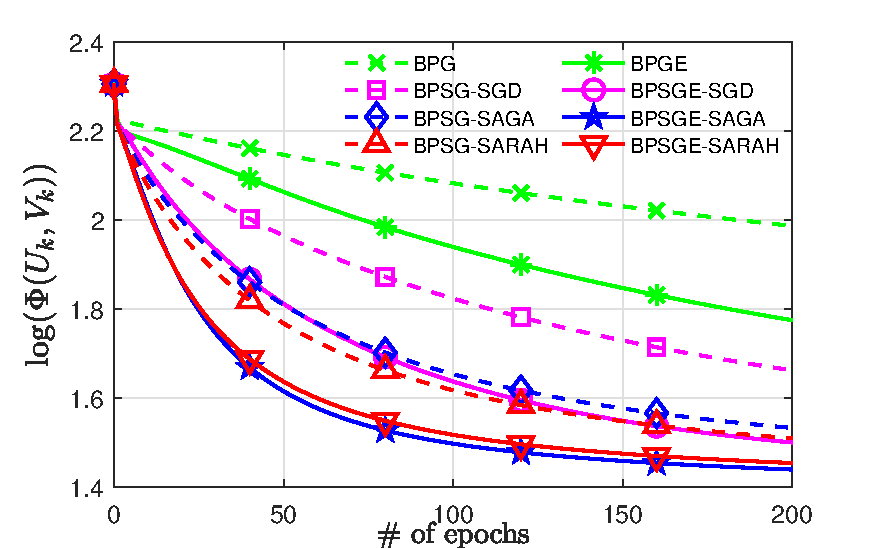
\includegraphics[width=0.485\textwidth]{SSNMF_ORL_epochs_23.png}
	% 		&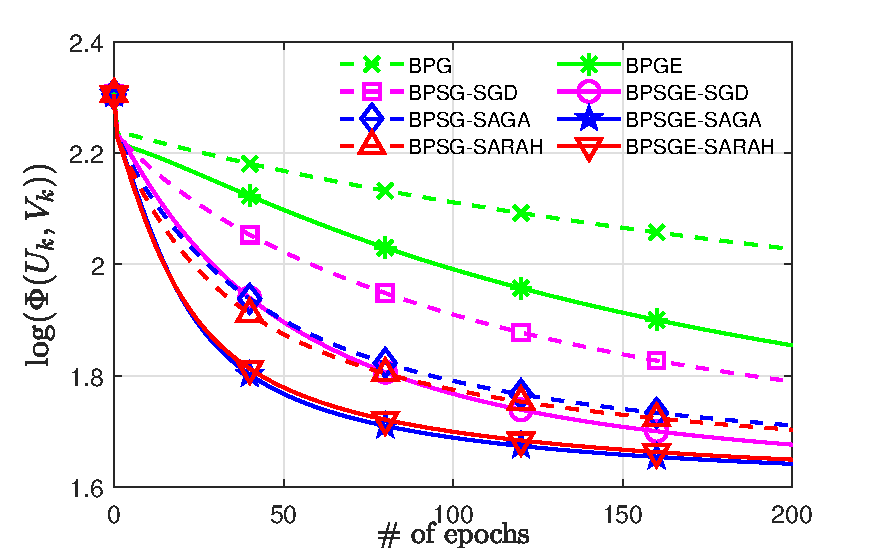
\includegraphics[width=0.485\textwidth]{SSNMF_ORL_epochs_25.png}\\
	% 		(a) $s_{1}=\frac{m}{2}$ and $s_{2}=\frac{d}{3}$&(b) $s_{1}=\frac{m}{2}$ and $s_{2}=\frac{d}{5}$\\
	% 		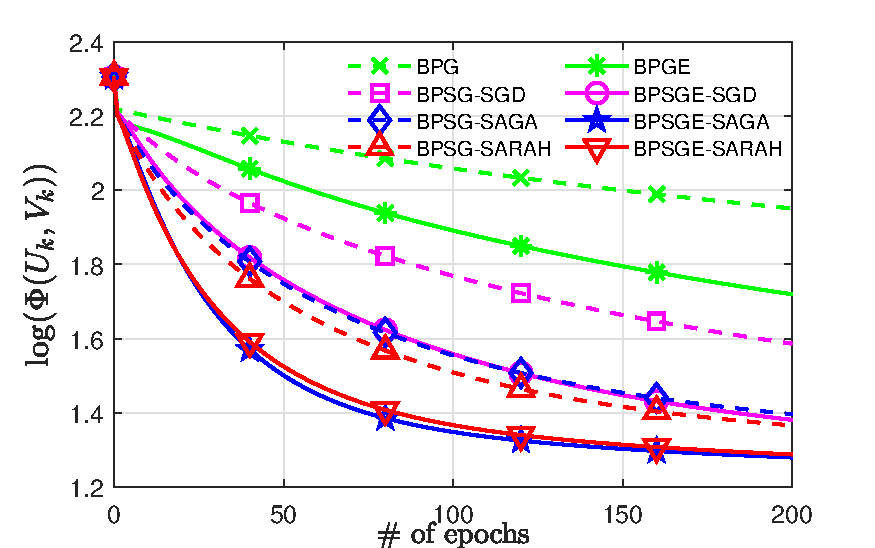
\includegraphics[width=0.485\textwidth]{SSNMF_ORL_epochs_22.png}
	% 		&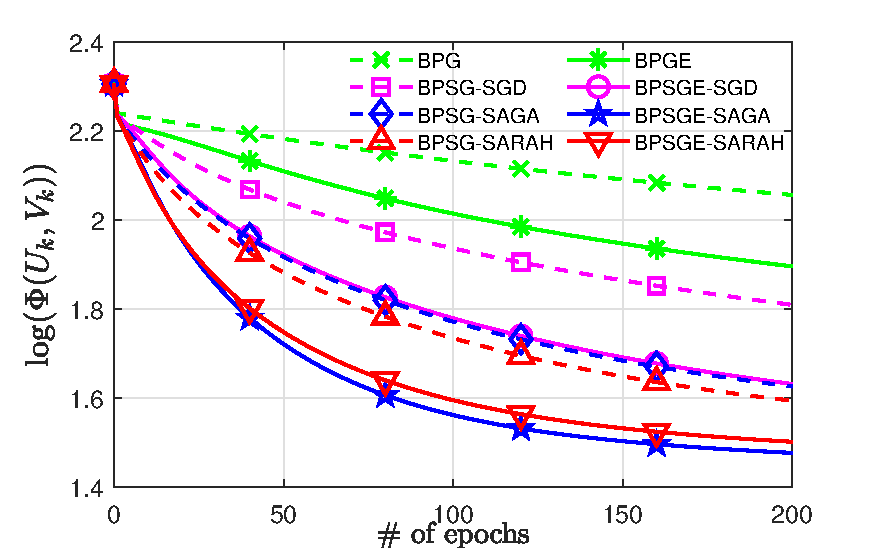
\includegraphics[width=0.485\textwidth]{SSNMF_ORL_epochs_32.png}\\
	% 		(c) $s_{1}=\frac{m}{2}$ and $s_{2}=\frac{d}{2}$&(d) $s_{1}=\frac{m}{3}$ and $s_{2}=\frac{d}{2}$
	% 	\end{tabular}
	% 	\caption{Numerical experiments for solving nonconvex sparse NMF problem \eqref{SSNMF}   on \emph{ORL} dataset with different $s_{1}$ and $s_{2}$. Top row: fixed $s_{1}$ and different $s_{2}$. Button row: different $s_{1}$ and fixed $s_{2}$.}
	% 	\label{SSNMF_epochs}
	% \end{figure}

	% The \emph{ORL} dataset with a reduced dimension of $r=25$ is utilized to demonstrate the efficiency of the proposed algorithm on the optimization problem \eqref{SSNMF}. All algorithms are run for $200$ epochs, with a subsampling rate of $5\%$ for stochastic algorithms. Figure \ref{SSNMF_epochs} compares the mean of the log of the objective function $\Phi(U_{k}, V_{k})$ versus the number of epochs for various algorithms, including BPG, BPGE, BPSG-SGD/SAGA/SARAH, and BPSGE-SGD/SAGA/SARAH.
	% %The first row of the figure displays the results with different values of $s_{1}$ and a fixed $s_{2}$, while the second row shows the results with a fixed $s_{1}$ and different values of $s_{2}$.



	% The results in Figure \ref{SSNMF_epochs} show that the BPGE algorithm outperforms the BPG algorithm, thanks to its extrapolation technique.The stochastic gradient algorithms that use the SAGA/SARAH estimator (BPSGE-SAGA/SARAH) perform better than their deterministic counterparts and the SGD estimator (BPSGE-SGD). The variance reduction technique also proves to be effective in the stochastic framework. Overall, the extrapolation technique speeds up convergence and the BPSGE-SAGA/SARAH algorithm provides the best results.

	The basis images generated by solving the nonconvex sparsity constrained NMF problem \eqref{SSNMF} for $s_{1}=\frac{m}{3}$ and $s_{2}=\frac{d}{2}$ are shown in Figure \ref{basis_SSNMF_ORL_32}. It validates the BPSGE algorithm outperforms other determinant algorithms and stochastic algorithms without extrapolation.

	\begin{figure*}[!ht]
		\setlength\tabcolsep{1pt}
		\centering
		\begin{tabular}{cccc}
			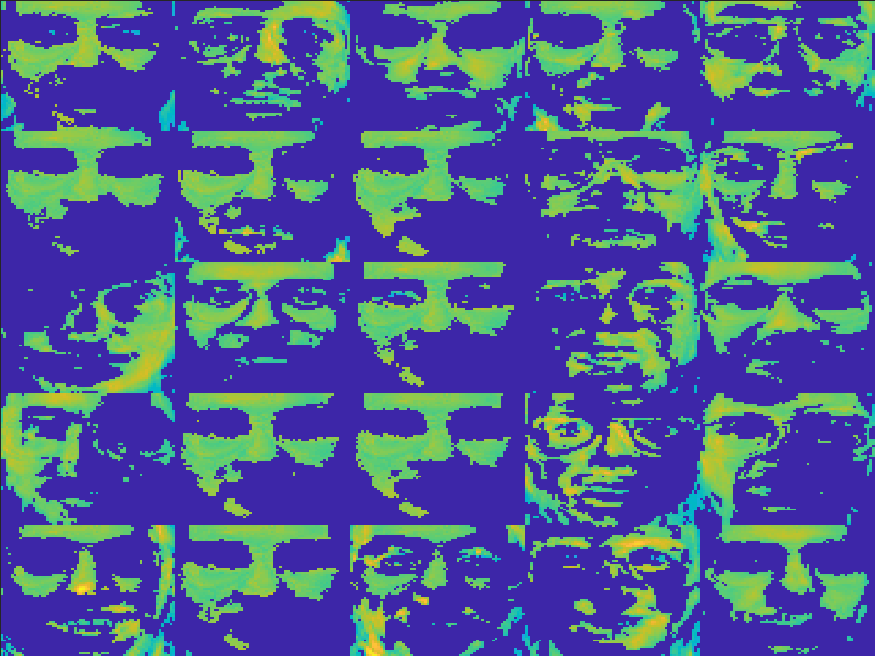
\includegraphics[width=0.24\textwidth]{figs/ORL_32_BPG}
			&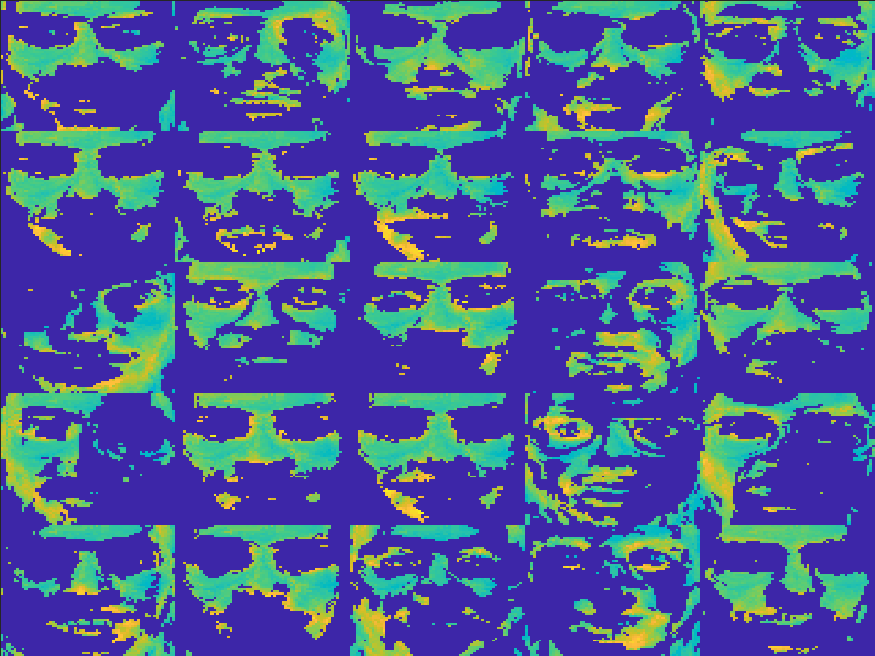
\includegraphics[width=0.24\textwidth]{figs/ORL_32_BPSG_SGD}
			&
\includegraphics[width=0.24\textwidth]{figs/ORL_32_BPSG_SAGA}
			&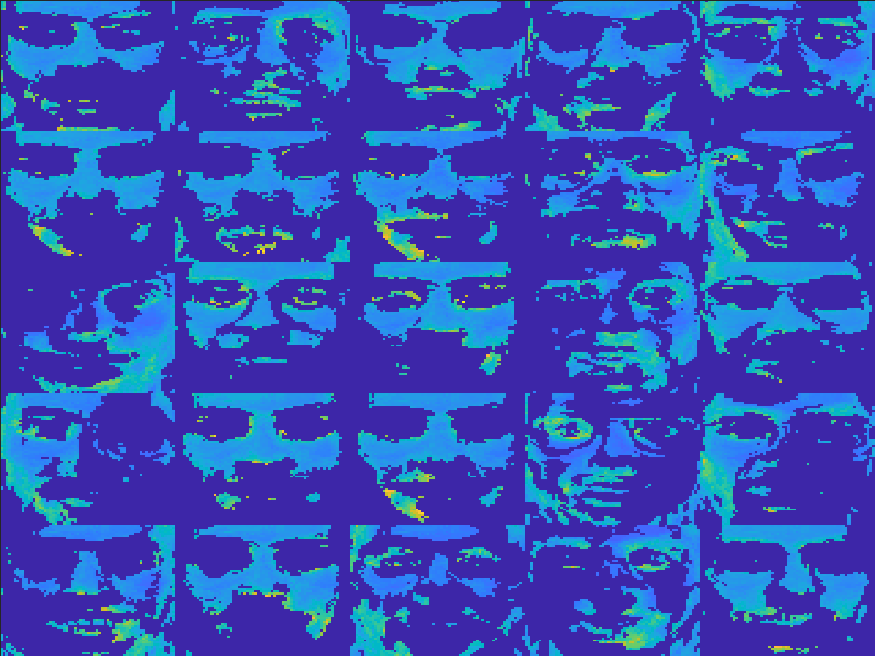
\includegraphics[width=0.24\textwidth]{figs/ORL_32_BPSG_SARAH}\\
			(a)BPG&(b)BPSG-SGD&(c)BPSG-SAGA&(d)BPSG-SARAH\\
			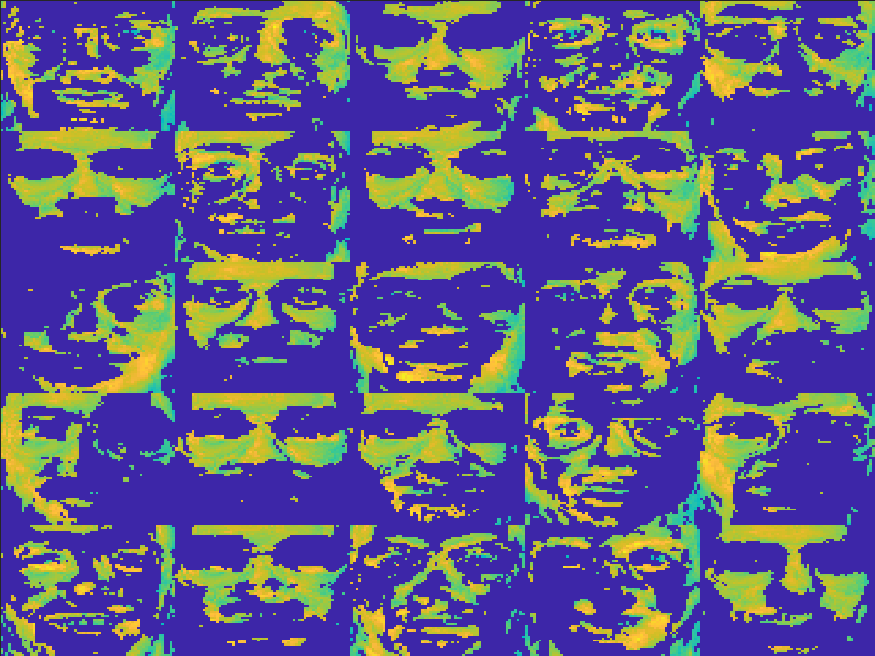
\includegraphics[width=0.24\textwidth]{figs/ORL_32_BPGE}
			&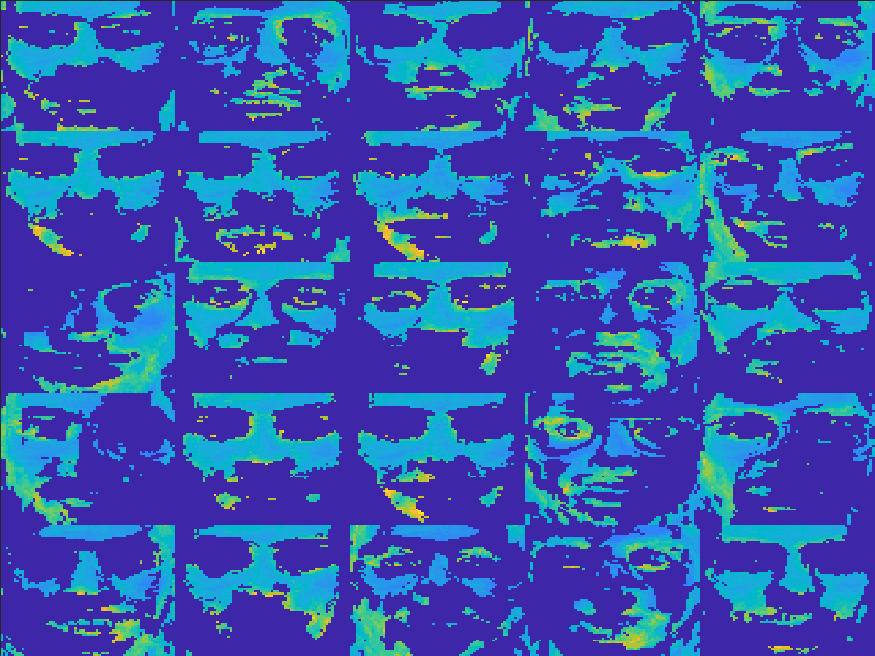
\includegraphics[width=0.24\textwidth]{figs/ORL_32_BPSGE_SGD}
			&
\includegraphics[width=0.24\textwidth]{figs/ORL_32_BPSGE_SAGA}
			&
\includegraphics[width=0.24\textwidth]{figs/ORL_32_BPSGE_SARAH}\\
			(e)BPGE&(f) BPSGE-SGD&(g)BPSGE-SAGA&(h)BPSGE-SARAH
		\end{tabular}
		\caption{The basis images generated by solving the nonconvex sparsity constrained NMF problem \eqref{SSNMF}  with $s_{1}=\frac{m}{3}$ and $s_{2}=\frac{d}{2}$.}
		\label{basis_SSNMF_ORL_32}
	\end{figure*}

\end{document}